% Copyright (c) 2021-2024 Michael Kuhn
%
% Permission to use, copy, modify, and/or distribute this software for any
% purpose with or without fee is hereby granted.
%
% THE SOFTWARE IS PROVIDED "AS IS" AND THE AUTHOR DISCLAIMS ALL WARRANTIES WITH
% REGARD TO THIS SOFTWARE INCLUDING ALL IMPLIED WARRANTIES OF MERCHANTABILITY
% AND FITNESS. IN NO EVENT SHALL THE AUTHOR BE LIABLE FOR ANY SPECIAL, DIRECT,
% INDIRECT, OR CONSEQUENTIAL DAMAGES OR ANY DAMAGES WHATSOEVER RESULTING FROM
% LOSS OF USE, DATA OR PROFITS, WHETHER IN AN ACTION OF CONTRACT, NEGLIGENCE OR
% OTHER TORTIOUS ACTION, ARISING OUT OF OR IN CONNECTION WITH THE USE OR
% PERFORMANCE OF THIS SOFTWARE.



\documentclass[
  12pt,
  a4paper,
  printlength,
  bibliography=totoc,
  chapterprefix,
  headings=openright,
  numbers=endperiod,
  parskip=half,
  twoside
]{scrreprt}
\usepackage[T1]{fontenc}
\usepackage[utf8]{inputenc}

\usepackage[ngerman]{babel}

% Enabling caching causes problems with overleaf..
\usepackage{minted}
\raggedbottom


\setminted{
  linenos=true,
  breaklines=true,
  frame=single,
  stripnl=true,
  numbersep=5px,
  breakanywhere=true,
  breakbefore=.-\,,
  ignorelexererrors=true,
}

\usepackage{xcolor}

\usepackage{pgfplots}

\usepackage{placeins}

\usepackage[citestyle=alphabetic,bibstyle=authortitle,hyperref=true,backref=true]{biblatex}
\addbibresource{thesis.bib}

%\usepackage{ellipsis, ragged2e, marginnote}
\usepackage{lmodern}
\usepackage{newtxmath}


\usepackage{tabularx}
\usepackage{longtable} %needs package ninecolors.sty
\usepackage{booktabs}
\usepackage[l3]{csvsimple} % or "\usepackage{csvsimple-l3}"

\usepackage{svg}
\svgsetup{inkscapepath=svgsubdir}

\usepackage{multicol}

\usepackage{microtype}
\usepackage[abspath]{currfile}

% Enable robust externalize for embedding images via url
\usepackage{robust-externalize}
\robExtConfigure{
  enable fallback to manual mode,
}

\usepackage{nicematrix}


% Use less space for the page number
\usepackage[margin=2.5cm,footskip=36pt,marginparwidth=2cm]{geometry}
\usepackage{graphicx}
%\usepackage[htt]{hyphenat}
\usepackage{microtype}
\usepackage{subcaption}
\usepackage[color=ovgu-orange,textwidth=\marginparwidth]{todonotes}

\usepackage{lipsum}

\usepackage{ifdraft}

% Used to get proper quotation style
\usepackage{csquotes}
\MakeOuterQuote{"}

\usepackage[hidelinks]{hyperref}
\usepackage[capitalise,noabbrev,german]{cleveref}


\graphicspath{{./figures/}}

\definecolor{ovgu-blue}{HTML}{0068B4}
\definecolor{ovgu-darkgray}{HTML}{606060}
\definecolor{ovgu-lightgray}{HTML}{C0C0C0}
\definecolor{ovgu-orange}{HTML}{F39100}
\definecolor{ovgu-purple}{HTML}{7A003F}
\definecolor{ovgu-red}{HTML}{D13F58}

\titlehead{\centering
\includegraphics[width=0.66\textwidth]{OVGU-INF}}

\subject{Bachelorarbeit}
\title{Containerisierte Client-Server-Applikationen für Hochleistungsrechner: Implementierung und Evaluation einer containerisierten JULEA-Installation}

\author{
  Finn Hering\\
  {\large\href{mailto:finn.hering@st.ovgu.de}{\nolinkurl{finn.hering@st.ovgu.de}}}
}

\date{\today}

\publishers{
  First Reviewer:\\
  Prof. Dr. Musterfrau

  \medskip

  Second Reviewer:\\
  Prof. Dr. Mustermann

  \medskip

  Supervisor:\\
  Dr. Evil
}

\begin{document}

\sloppy

% \frontmatter
\pagenumbering{roman}

\maketitle

\begin{abstract}
Die immer steigende Rechenleistung hat zur Folge, dass in der Wissenschaft und insbesondere im High Performance Computing (HPC) Bereich die Komplexität der Problemstellung aufgrund der erhöhten Rechen-Ressourcen steigen. Dies hat zur Folge, dass somit auch die Applikationen, welche diese Problemstellungen lösen komplexer werden. Komplexe Applikationen haben oft viele direkte oder indirekte Abhängigkeiten und Systemvoraussetzung, welche das manuelle Ausrollen der Applikation sehr fehlernanfällig und zeitaufwendig machen. 

Um das Problem des Ausrollens von komplexen Applikationen zu minimieren, wird in dieser Arbeit anhand einer Beispielapplikation – "JULEA" – eine referenzimplementierung der Containerisierung modelliert und implementiert. Anschließend wird die Performance der Containersierung von JULEA anhand eines Apptainer Container im vergleich zu der nativen Installation von JULEA auf einem HPC-System evaluiert.

Die Ergebnisse zeigen, dass die Containerisierung von JULEA keine signifikanten Performance-Einbußen hat und die Containerisierung von JULEA eine gute Alternative zur nativen Installation von JULEA ist. Die Containerisierung von JULEA hat den Vorteil, dass die Installation von JULEA auf einem HPC-System vereinfacht und reproduzierbar wird. Außerdem wird dem ausrollenden das Kompilieren der Abhängigkeiten für JULEA abgenommen, da die Abhängigkeiten mit dem Containerimage mitgeliefert werden.
\end{abstract}

\tableofcontents



% \mainmatter

\ifdraft{\cleardoubleoddpage}{}
\pagenumbering{arabic}

% Einleitung
\chapter{Einführung}
\label{cha:introduction}

\section{Motivation}
Im Jahr 2022 überstieg der erste Supercomputer – "Frontier" – die 1-ExaFLOP-Marke \cite[Vgl. S. 567ff]{rajaramanFrontierWorldsFirst2023}. Dies ist ein Meilenstein der HPC-Entwicklung und bringt neue Möglichkeiten für die Forschung und Wissenschaft.

Die immer steigende Rechenleistung in fast allen Bereichen der Informationstechnologie – nicht nur im HPC-Bereich – ermöglicht es, Applikationen mit immer steigenden Anforderungen und Komplexität zu entwickeln. Dies ermöglicht die Lösung immer komplexerer Probleme. Ein Indiz für die steigende Komplexität von Applikationen kann die Anzahl verwendeter Abhängigkeiten sein, welche die Komplexität der Applikation auf Code Dritter auslagern \cite[Vgl. Abbildung 2.4]{sonatype2024StateSoftware}. Die Verwendung von Abhängigkeiten birgt einige logistische Probleme. Eines dieser logistischen Probleme ist das Ausrollen von Applikationen in heterogenen Umgebungen, das mit steigender Anzahl von Abhängigkeiten weiter erschwert wird. Um das Problem zu minimieren, können Virtualisierungstechnologien immens helfen. Virtualisierungstechnologien ermöglichen es auf heterogenen Systemen eine homogene Umgebung zu schaffen. Diese kann dann als Basis für die Applikation dienen und eine einfach replizierbare Ausrollung schaffen. Davon profitieren nicht nur die Systemadministratoren und die Endanwender, sondern auch die Entwickler, welche die virtualisierte Umgebung für die Entwicklung nutzen können. Das erspart den Entwicklern das Aufsetzen einer eigenen Entwicklungsumgebung, was durchaus zeitintensiv sein kann. Bei der Virtualisierung gibt es zweierlei populäre Technologien: Containervirtualisierung und Hardwarevirtualisierung.

\section{Ziel der Arbeit} \label{sec:ziel-der-arbeit}

Das Ziel dieser Arbeit ist es, die Containervirtualisierung einer komplexeren Applikation – JULEA – zu implementieren und zu untersuchen. JULEA \cite{kuhnJULEAFlexibleStorage2017} ist ein Framework, das arbiträre Client-Schnittstellen und eine hohe Flexibilität bietet, um das Evaluieren verschiedener Speicher-Lösungen und Ansätze zu beschleunigen \cite[Vgl. S. 1]{kuhnJULEAFlexibleStorage2017}. JULEA ist eine Applikation, die viele Abhängigkeiten hat und eignet sich daher gut für die Untersuchung der Containervirtualisierung.

Die drei zentralen Fragen, welche mit dieser Arbeit beantwortet werden sollen, sind:

Kann die Containerisierung von JULEA die Performance von JULEA beeinflussen? \\
Ist es möglich HPC-Anwendungen – wie JULEA – zu Containerisieren? \\
Ist es möglich für JULEA Entwicklungscontainer mit bereits kompilierten Abhängigkeiten zu erstellen?

\section{Struktur der Arbeit}

Die Arbeit wird folgendermaßen strukturiert sein:

\paragraph{Hintergrund}

Im Hintergrund (\cref{cha:background}) werden alle verwendeten Technologien und Konzepte, welche für das Verständnis der Arbeit notwendig sind, erläutert.

\paragraph{Implementierung und Design}

In der Implementierung und Design (\cref{cha:implementation_design}) wird die Implementierung der Containerisierung von JULEA beschrieben und das Design der Containerisierung erläutert.

\paragraph{Evaluation}

In der Evaluation (\cref{cha:evaluation}) wird die Performance der Containerisierung von JULEA untersucht und mit der nativen Installation von JULEA verglichen.

\paragraph{Verwandte Arbeiten}

In den verwandten Arbeiten (\cref{cha:related-work}) werden Arbeiten vorgestellt, welche sich mit der Containerisierung von Applikationen beschäftigen und inwiefern diese Arbeiten sich von dieser Arbeit unterscheiden.

\paragraph{Fazit}

Im Fazit (\cref{cha:conclusion}) werden die Ergebnisse der Arbeit zusammengefasst und ein Ausblick auf mögliche zukünftige Arbeiten gegeben.



% Hintergrund
\chapter{Hintergrund}

\label{cha:background}
\textit{In diesem Kapitel werden die genutzten Technologien erläutert}

\section{Containervirtualisierung}

Containervisualisierung (auch Containerisierung genannt) beschreibt das Bereitstellen einer Applikation, indem die Applikation und alles, was diese zum Laufen benötigt ((System-)Bibliotheken, ausführbare Dateien, (System-)Konfigurationen, etc.) in Form eines Container-Images bereitgestellt wird. Das ermöglicht es, die Applikation isoliert, schnell und zuverlässig auf unterschiedlichen Host-Systemen auszuführen.

Im Gegensatz zur klassischen Virtualisierung wird nicht die Hardware-Ebene abstrahiert und ein komplett eigenständiges Betriebssystem hochgefahren, sondern lediglich die Betriebssystem-Ebene abstrahiert.

Das hat zur Folge, dass Containervirtualisierung weniger Speicher verbraucht und performanter im Vergleich zu Hardwarevirtualisierung ist.

\section{OCI-Container-Image Spezifikation}

Die Open Container Initiative (OCI) ist eine Organisation, welche sich auf die Standardisierung von Containern spezialisiert hat. Mitglieder dieser Initiative sind u.A. Microsoft, Amazon Web Services, Google und Red Hat. Die von OCI bereitgestellte Spezifikation definiert den aufbau eines Container-Images.

\section{ContainerD}

ContainerD ist ein System-Daemon, welcher die OCI-Image-Spezifikation unterstützt und die verwaltung Containern übernimmt. Docker nutzt ContainerD als Backend für die Containervisualisierung. Das Unternehmen hinter Docker hat ContainerD als Open-Source-Projekt veröffentlicht und arbeitet an diesem.

\begin{figure}[H]
    \includegraphicsWeb[width=\linewidth]{https://containerd.io/img/architecture.png}
    \captionof{figure}{ContainerD Architektur: https://containerd.io/img/architecture.png}
\end{figure}


ContainerD selber ist in mehrere Komponenten aufgeteilt. Diese beinhalten unter anderem:

Eine API um mit unterschiedlichen ContainerD-Clients (Frontends) zu kommunizieren. Hierzu zählen CRI und die native ContainerD-Schnistelle. CRI ist selber nur ein Wrapper um die native ContainerD-Schnistelle. Die CRI-Schnistelle wird größtenteils von Kzbernetes genutzt, um ContainerD zu steuern. Die native ContainerD-Schnistelle wird unter anderem von Docker genutzt.

Der ContainerD-Core, welcher alle nötigen Metadaten und funktionalitäten bereitstellt, um Container zu verwalten. Dieser kommuniziert wiederrum mit dem ContainerD-Backend.

Das ContainerD-Backend ist wiederrum für die eigentliche Ausführung der Container zuständig. Es abstrahiert die dafür nötigen OS-Funktionalitäten für den ContainerD-Core.

ContainerD benötigt erweiterte rechte auf dem Host-System. Aus diesem Grund läuft ContainerD standardmäßig als Root-Prozess. Es ist mlglich diesen ohne Root-Rechte zu verwenden, allerdings nur mit einem deutlichen Mehraufwand.

\section{Docker}

Docker ist eine der bekanntesten Containervisualisierungs-Lösungen. Sie beinhaltet eine Reihe von Werkzeugen zum Erstellen, verwalten und ausführen von Containern. Docker ist ein Frontend für ContainerD.

\subsection{Dockerfile}

Eine Dockerfile ist die Definition, welche Docker benötigt, um ein Container-Image zu erstellen. In ihr werden alle nötigen Schritte sowie Metainformation definiert, um einen Container mit einer lauffähigen Applikation zu haben. Die in der Dockerfile definierten Schritte werden isoliert auf einem Basis-Image ausgeführt. Das durch die Dockerfile erstelle Image ist somit das Resultat alle Schritte, aus dem das Basis-Image entsteht und den in der Dockerfile definierten Schritten.

Hier ist ein simples Dockerfile Beispiel für das Erstellen eines Julea Container-Images:

\inputminted{docker}{./code-examples/Dockerfile.example}

\subsection{OCI-Container-Image Layer}

Ein OCI-Container-Image setzt sich aus Schichten (Layer) zusammen, welche stapelweise angeordnet sind. In jeder Schicht werden Änderungen an der vorherigen Schicht vorgenommen. Jedes OCI-Container-Image hat ein sogenanntes "Base-Image". Dieses ist die erste Schicht. Ein "Base-Image" ist üblicherweise ein spezifisches Betriebssystem (z. B.: Debian, Ubuntu, Windows, etc.).

\subsection{Docker Build-Cache}

Docker verfügt über Caching-Mechanismen, welche subsequente Builds beschleunigen. Das Caching funktioniert, indem Docker jedes einzelne "Layer" zwischenspeichert. Wenn sich ein Layer ändert, müssen nur die Layer, welche direkt oder indirekt auf dem Layer aufbauen, neu ausgeführt werden. Um das caching möglichst effektiv zu verwenden, sollte man also sicherstellen, dass Layer, welche besonders lange zum Erstellen brauchen, möglichst nur dann neu erstellt werden, wenn dies auch notwendig ist.

\subsection{Docker BuildKit}

Docker BuildKit ist das neue Backend um OCI-Container-Images mit Docker zu erstellen. Ziel von BuildKit ist es, den Docker Legacy Builder zu ersetzen.

Docker BuildKit hat viele Verbesserungen, um Docker Builds, im Vergleich zum Docker Legacy Builder, performanter zu machen. Dazu zählen: Parallelisierung von Build-Stages, Auslassen von unbenutzten Build-Stages, mehr Caching Möglichkeiten wie z. B. Cache-Mounts, u. v. m.

Docker BuildKit Backends müssen nicht explizit auf dem Computer installiert werden, auf dem man entwickelt. Docker kann auch BuildKit Backend von Remote-Servern einbinden. Das ermöglicht es, Builds auf leistungsstärkeren Servern, sowie auf Servern mit einer anderen CPU-Architektur auszuführen, um die Build-Zeit zu verkürzen.

\subsubsection{Docker Buildx}

Um das Docker BuildKit Backend mit Docker zu verwenden, nutzt man Docker Buildx. Docker Buildx ist eine offizielle Docker Erweiterung. Docker Buildx hat einige Funktionalitäten um Docker BuildKit Backends einzubinden, sowie festzulegen welche BuildKit Backends man verwenden möchte.

\subsubsection{Docker Buildx Bake}

Eine weitere Funktionalität von Docker Buildx ist Docker Buildx Bake. Docker Buildx Bake ermöglicht es mithilfe einer sog. Bakefile das erstellen und mehrerer OCI-Container-Images zu vereinfachen.

Momentan wird Julea in mehreren Ubuntu-Versionen sowie mit mehreren Compilern kompiliert und getestet. Somit müssten mehrere Dockerfiles ertellt werden, um alle Kombinationen zu testen. Mit Docker Buildx Bake kann man das Erstellen mehrerer Docker-Container-Images vereinfachen.

\inputminted{./lexers/docker-bake-lexer.py}{./code-examples/docker-bake.example.hcl}

\section{Container-Images für Entwicklungsumgebungen}

Während sich die "klassische" Containerisierung darauf fokussiert eine produktive Applikation zuverlässig auszurollen, fokussieren sich die Container-Images für Entwicklungsumgebungen darauf Entwicklern eine einheitliche Container-Umgebung zum Testen und Entwickeln bereitzustellen. Im Idealfall sollte ein Entwicklungs-Container den einstieg in ein Projekt/eine Entwicklungsumgebung erleichtern, indem im Container bereits alles eingerichtet ist, um an einem Projekt effektiv zu arbeiten.

Solche Container-Images sollten alle nötigen Abhängigkeiten, welche man zum Entwickeln benötigt, enthalten. Dazu zählen z. B. Compiler, Interpreter, Bibliotheken, Tools.

Im fall von Julea muss ein solcher Entwicklungs-Container alle Abhängigkeiten enthalten, um an oder mit Julea zu entwickeln. Diese Abhängigkeiten müssen kompiliert werden. Das Kompilieren ist sehr zeitaufwendig. Darum sollte ein fertiges Container-Image diese Abhängigkeiten beinhalten, sodass das initiale Kompilieren der Abhängigkeiten übersprungen werden kann.

Ein Container-Image alleine müsste allerdings immernoch vom Entwickler selber in den Editor/IDE integriert werden, da das Denutzen des Containers sonst sehr aufwändig wär. Um die integration in den Editor/IDE zu vereinfachen, bietet Microsoft eine offene Spezifikation ("Development Container") an. Wenn ein Editor/IDE diese Spezifikation unterstützt, kann der Entwickler mit einem Klick den Container in den Editor/IDE integrieren.

Neben der einfachen Integration in den Editor/IDE ermöglicht die Spezifikation eine reihe an einstellungsmöglichkeiten. So kann der Entwickler z. B. festlegen, welche Extensions installiert werden sollen, welche Umgebungsvariablen gesetzt werden sollen, welche Ports nach außen freigegeben werden sollen, welche Editor/IDE-Einstellungen gesetzt werden sollen, u. v. m.


\subsection{Editor/IDE-Unterstützung}

\begin{table}[H]
    \begin{NiceTabular}{X|X|X[4]}[hlines]
        IDE/Editor Name    & Unterstützung & Anmerkung \\
        Visual Studio Code & Ja            & Vollständige Unterstützung                                                                                                                                                                                              \\
        CLI                & Ja            & Es existiert ein offizielles CLI in form eines NPM-Paketes @devcontainer/cli. Dadurch ist es auch möglich \(Neo-\)VIM und andere Terminal-Texteditoren mit Devcontainern zu verwenden                                   \\
        Visual Studio      & Ja*           & Stand 01.12.2024: Eigeschränkte unterstützung. Aktuell sind nur C++-Projekte mit CMake unterstützt                                                                                                                      \\
        JetBrains IDEs     & Ja*           & Stand 01.12.2024 ist die unterstützung in der Beta-Phase und unvollständig.                                                                                                                                             \\
        VIM                & Ja*           & Stand 01.12.2024 gibt es ein community plugin für Neo-VIM welches devcontainer integration ermöglicht. Die vollständigkeit dieses Plugins wurde nicht überprüft. Siehe: https://codeberg.org/esensar/nvim-dev-container \\
        Sublime Text       & Nein          & Stand 01.12.2024: Es gibt keine offizielle Aussage, ob oder wann es eine Devcontainer unterstzüng geben soll                                                                                                            \\
        Eclipse            & Nein          & Stand 01.12.2024: Es gibt keine offizielle Aussage, ob oder wann es eine Devcontainer unterstzüng geben soll                                                                                                            \\
        Netbeans           & Nein          & Stand 01.12.2024: Es gibt keine offizielle Aussage, ob oder wann es eine Devcontainer unterstzüng geben soll                                                                                                            \\
        Code::Blocks       & Nein          & Stand 01.12.2024: Es gibt keine offizielle Aussage, ob oder wann es eine Devcontainer unterstzüng geben soll                                                                                                            \\
        Notepad++          & Nein          & Stand 01.12.2024: Es gibt keine offizielle Aussage, ob oder wann es eine Devcontainer unterstzüng geben soll                                                                                                            \\
        Emacs              & Nein          & Stand 01.12.2024: Es gibt keine offizielle Aussage, ob oder wann es eine Devcontainer unterstzüng geben soll                                                                                                            \\
    \end{NiceTabular}
\end{table}

\section{Apptainer (früher: Singularity)}

Apptainer ist eine alternative Container-Lösung. Sie nutzt im Gegensatz zu Docker keine OCI-Container-Images, kann diese aber konvertieren. Apptainer-Container-Images werden als einzelne Datei gespeichert, das erleitert das Verteilen des Container-Images ohne einen Registry-Server. Es werden keine erweiterten Berechtigungen durch Apptainer benötigt, um Container auszuführen. Dies ist insbesondere für HPC-Umgebungen relevant, da das Ausführen von Applikationen als root-Benutzer hier ungewöhnlich ist.

\section{CI/CD}

\begin{figure}[H]
    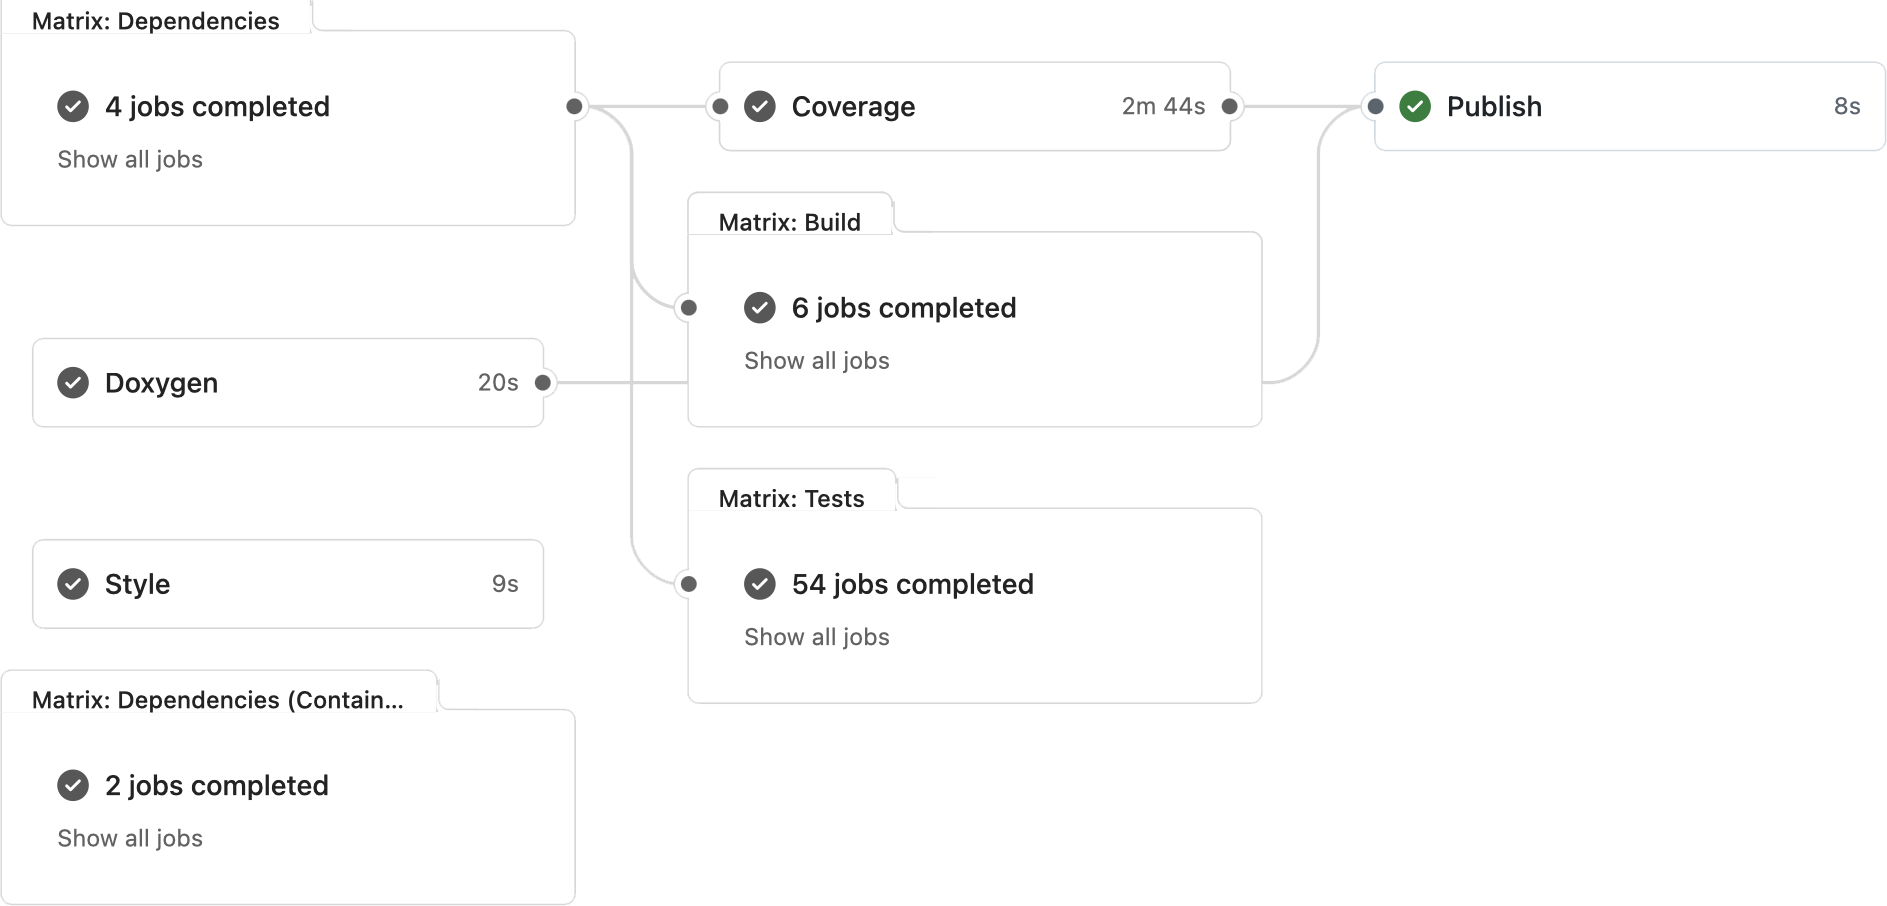
\includegraphics[width=\textwidth]{julea-ci-cd-full.png}
    \caption{CI/CD-Pipeline von Julea. \newline
        Siehe: https://github.com/parcio/julea/actions/runs/8318540808}
\end{figure}

CI/CD, auch CI/CD-Pipeline genannt, ist die Kombination von Contiguous Integration (CI) und Contiguous Deployment/Contiguous Delivery (CD). Eine CI/CD-Pipeline ist eine automatisierte Abfolge von Schritten, welche das Testen, Kompilieren, Bereitstellen und Ausrollen von Artefakten automatisiert. Oftmals sind solche CI/CD-Pipelines direkt teil einer modernen Versiom-Control-System-Plattform wie z. B. GitHub, GitLab, BitBucket, etc. und regieren somit vollautomatisch auf Code-Änderungen.

\subsection{Contiguous Integration (CI)}

Unter Contiguous Integration (CI) versteht man unter anderem das automatisierte testen und/oder kompilieren von Code.  Dieser automatismus dient dazu den Software-Entwickern Zeit zu erspaaren, wodurch sie sich auf das eigentliche entwickeln fokussieren können.

Im gezeigten Beispiel gehören alle bis auf den letzten Schritt "Publish" zur Contiguous Integration (CI).

\begin{figure}[H]
    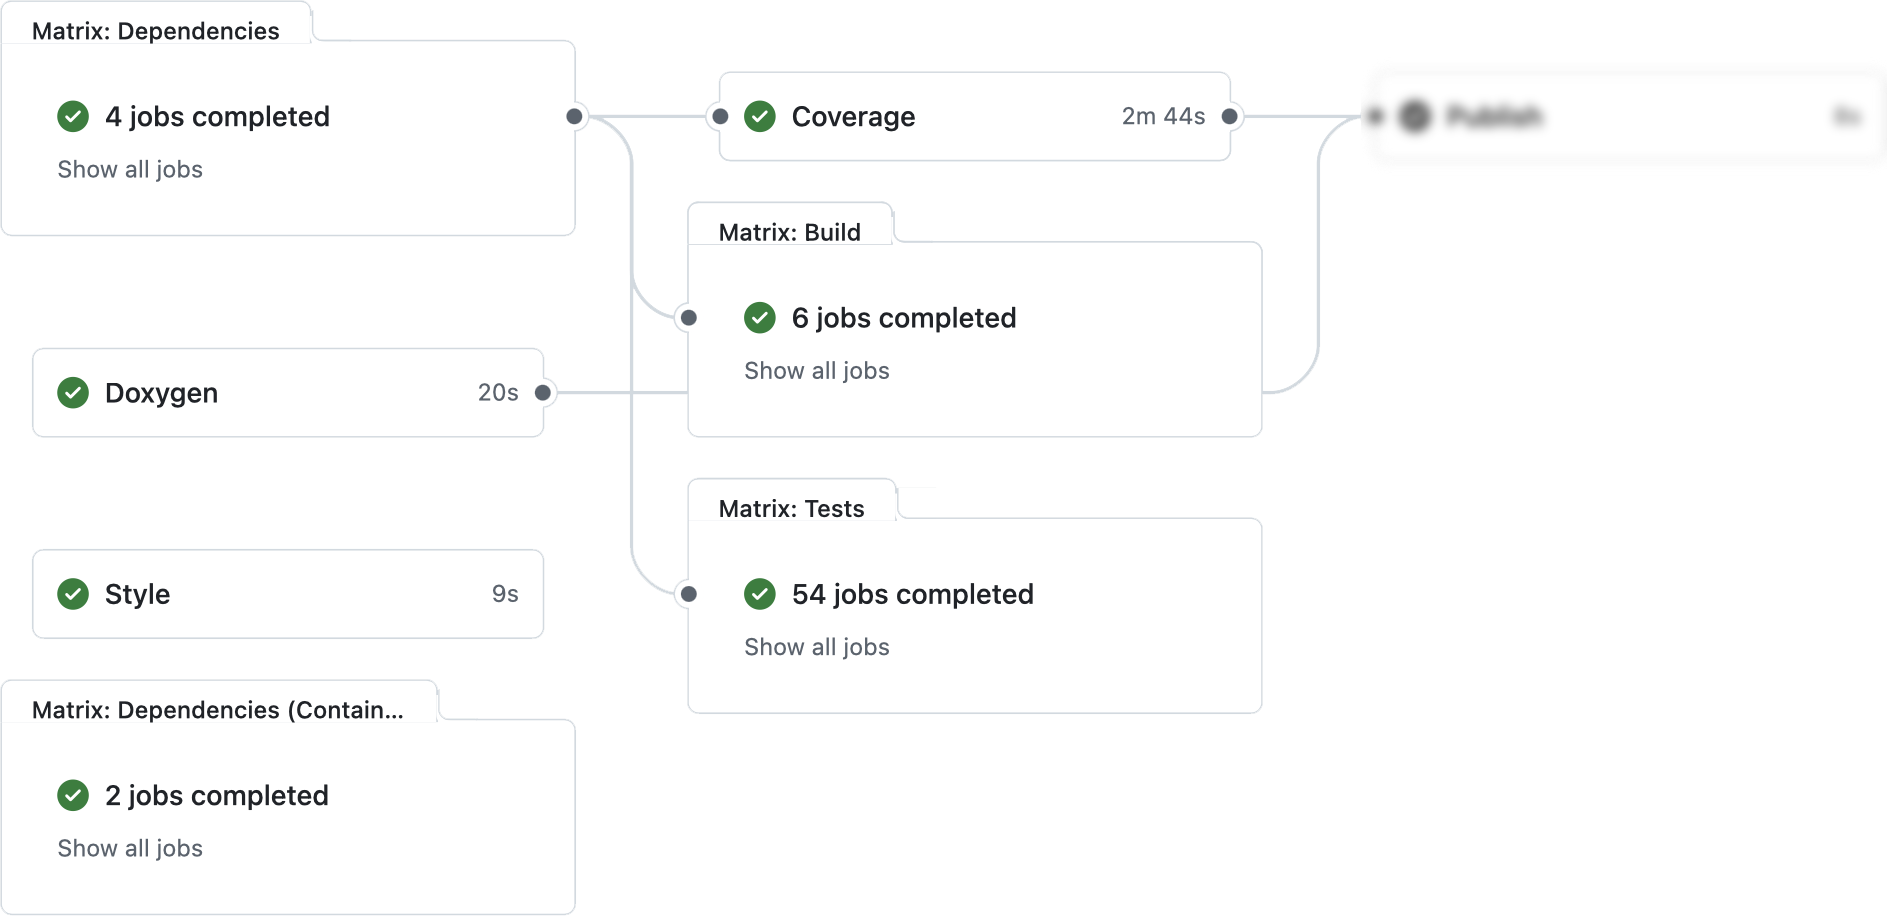
\includegraphics[width=\textwidth]{julea-ci-cd-ci-focus.png}
    \caption{CI/CD-Pipeline von Julea. \newline
        Siehe: https://github.com/parcio/julea/actions/runs/8318540808}
\end{figure}

\subsection{Contiguous Delivery (CD)}

Unter Contiguous Deployment (CD) versteht man das automatisierte bereitstellen von Artefakt. Üblicherweise sind Artefakte Container-Images, ausführbare Dataien, Archive, etc.

Im gezeigten Beispiel gehört nur der letzte Schritt "Publish" zu Contiguous Delivery (CD). In diesem Schritt wird die Dokumentation von Julea automatisch veröffentlicht.

\begin{figure}[H]
    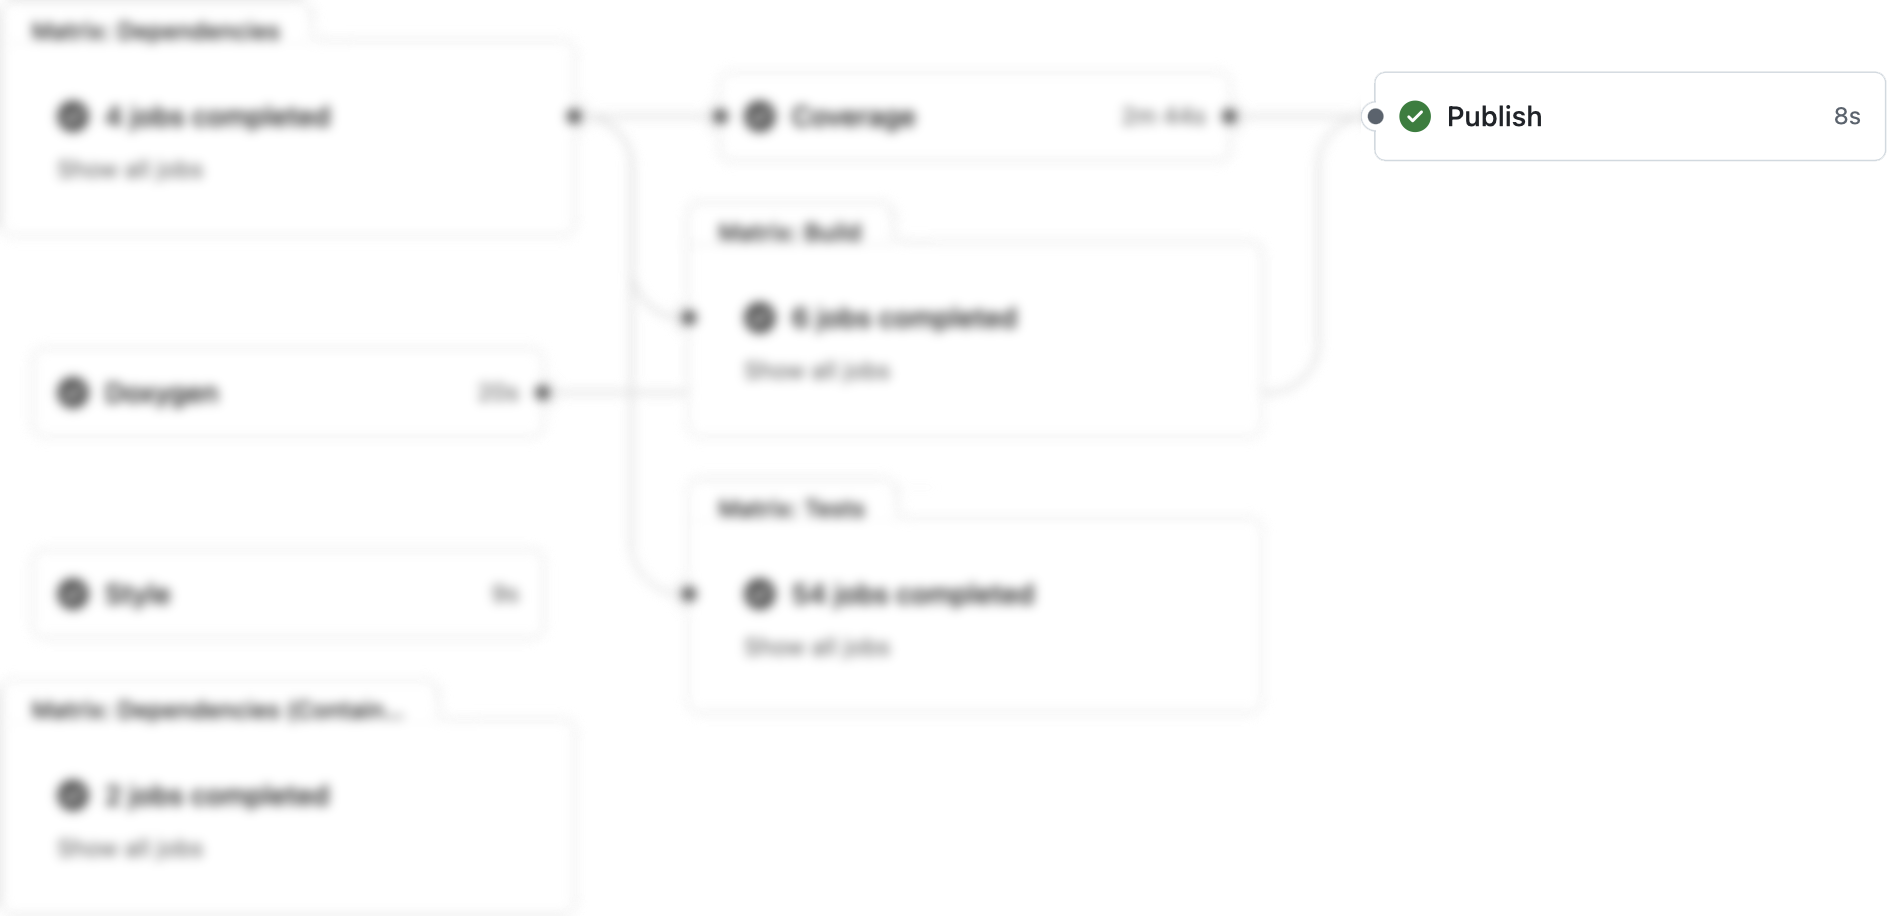
\includegraphics[width=\textwidth]{julea-ci-cd-cd-focus.png}
    \caption{CI/CD-Pipeline von Julea. \newline
        Siehe: https://github.com/parcio/julea/actions/runs/8318540808}
\end{figure}

\subsection{Contiguous Deployment (CD)}

Unter Contiguous Deployment (CD) nimmt das konzept von Contiguous Delivery (CD) auf und rollt das bereitgestellte Artefakt automatisiert aus. In der regel wird das paket auf eine Testumgebung ausgerollt, um sicherzustellen, dass das Artefakt auch tatsächlich stabil lauffähig ist. In der umgebung werden in der Regel automatisierte und/order manuelle Integrationtests durchgeführt. Sollten die tests erfolgreich sein, wird das artefakt sofort oder zu einem release-zeitpunkt auf die Produktivumgebung ausgerollt.

\subsection{GitHub-Actions}

Github-Actions (GHA) ist die GitHub-eigene CI/CD-Pipeline-Lösung. GitHub-Actions ermöglicht es mithilfe einer YML-Datei CI/CD-Pipelines zu definieren. Diese YML-Datei wird im Repository abgelegt und von GitHub-Actions ausgeführt. GitHub-Actions bietet eine Vielzahl von Funktionsbausteinen, welche häufig in CI/CD-Pipelines benötigt werden in einer abstrahierten Form an. Diese bausteine werden entweder von GitHub oder Dritten zur verfügung gestellt. Die bausteine werden in einer isolierten Container-Umgebung ausgeführt, um möglichst reproduzierbare Ergebnisse zu erzielen.

GitHub-Actions werden als teil dieser Arbeit genutzt, um automatisiert die Julea-Container-Images zu erstellen und zu veröffentlichen.

Diese pipeline baut und veröffentlicht ein Dockerimage, immer wenn ein neuer commit in die "master" Branch gepusht wurde:
\inputminted{yaml}{./code-examples/gha.yml} 

\section{Julea}

In dieser Arbeit wird Julea als Beispiel für eine Applikation verwendet, welche in einem Container-Image bereitgestellt werden soll. Julea ist ein Speicher-Framework, welches mehrere Speicher-Backends wie z. B. Datei-Speicher, MySQL, MongoDB, u. v. m. unterstützt. Julea ist ein Open-Source-Projekt und wird von der Arbeitsgruppe "Parallel Computing and I/O" an der Otto-von-Guericke-Universität Magdeburg entwickelt.

Der Quellcode von Julea wird auf GitHub bereitgestellt: \url{https://github.com/parcio/julea}

\section{HPC}

HPC steht für High Performance Computing. HPC-Systeme sind spezielle Computer-Systeme, welche besonders leistungsstark sind. HPC-Systeme werden für berechgnungen mit besonders hohen CPU oder Speicheranforderungen genutzt. Oft werden HPC-Systeme in Forschungseinrichtungen, Universitäten, oder in der Industrie genutzt. HPC-Applikationen sind häufig hochkomplex und greifein auf große mengen von Abhängigkeiten zurück, welche entweder zur Kompilierungszeit, oder zur Laufzeit benötigt werden. Eine hohe anzahl an Abhängigkeiten erschwert das Erstellen von reproduzierbaren Laufzeit-, sowie Kompilierungsergebnissen, da die mögliche kombination von Abhängigkeiten, welche zur Laufzeit und/oder zur Kompilierzeit benötigt werden. 

Die Komplexität von Abhängigkeiten in einer Applikation lässt sich folgendermaßen moddellieren:
\begin{flalign*}
    &\text{Sei } D_a = (x_0,\dots, x_n), x_i \in \mathbb{N} \\&
    \text{und } x_i \text{ die Anzahl der akzeptierten Variationen der }i\text{-ten Abhängigkeit der Applikation } a&
\end{flalign*}
Dann ist die Anzahl der unterschiedlichen Umgebunden, in der die Applikation $a$ funktionieren sollte: 
\begin{align*}
   \prod_{i=0}^{|D_a|} x_i
\end{align*}

Angenommen, es gibt eine Applikation $b$, welche 3 Abhängigkeiten mit jeweils 3 akzeptierten varianten hat ($D_b = (3, 3, 3)$), dann ist: 
\begin{align*}
    \prod_{i=0}^{|D_b|} x_i &= \prod_{i=0}^{3} x_i\\
    &= 3 \cdot 3 \cdot 3 \\
    &= 27
\end{align*}

Seien:
\begin{align*}
    f(n) &= (x_i)_{i=0}^{n}, \text{wobei } n \in \mathbb{N} \text{ und } x_i = 3 \\
    g(n) &= \prod_{i=0}^{|f(n)|} f(n)
\end{align*}

Dann stellt $g(n)$ die Anzahl der unterschiedlichen Umgebungen für $n$ Abhängigkeiten mit jeweils 3 akzeptierten Variationen je Abhängigkeit dar:

\begin{tikzpicture}
    \begin{axis}[
        axis lines = left,
        xlabel = \(n\),
        ylabel = {\(g(n)\)},
    ]
    %Below the red parabola is defined
    \addplot [
        domain=0:6,
        samples=100, 
        color=red,
    ]
    {3^x};
    \addlegendentry{\(\prod_{i=0}^{|f(n)|} f(n)\)}
    
    \end{axis}
\end{tikzpicture}

Es wird ersichtlich, dass die Anzahl der unterschiedlichen Umgebungen exponentiell mit der Anzahl der akzeptierten Variationen wächst. 

Dies bedeutet, dass Applikationen, welche sehr viele Abhängigkeiten haben, und diese Abhängigkeiten selbst mehrere variationen (Versionen, Kompilierung-Flags, etc.) haben ist es unmöglich jede mögliche Umgebung zu testen. Es ist in diesen Fall einfacher eine möglich konsistente Umgebung zu schaffen. Übliche mechanismen eine solche konsistente Umgebung zu schaffen ist Virtualisierung oder das Eliminieren von mehreren akzeptierten Abhängigkeitsvariationen durch Version-Pinning. Hierbei ist allerdings zu beachten, dass Version-Pinning nicht indirekte Abhängigkeiten konsistent hält. Dies ist bei der Virtualisierung anders. Die Hardwarevirtualisierung stellt sicher, dass alles bis zur Hardware-Ebende konsistent gehalten werden kann, dies kommt üblicherweise mit performance-einbußen einher und einem großen Paket, welches ausgerollt werden müsste. Hier bietet die Containervisualisierung einen mittelweg, indem es alles bis zum Betriebssystem konsistent hält und somit kaum bis garkein Performanceoverhead, sowie eine – im Vergleich zur Hardwarevirtualisierung – kleinere Paketgröße.


% Verwandte Arbeiten Kapitel
\chapter{Verwandte Arbeiten}
\label{cha:related-work}
\textit{In diesem Kapitel werden verwandte Arbeiten vorgestellt}

\section{Containerizing CS50: Standardizing Students' Programming Environments \cite{malanContainerizingCS50Standardizing2024}}


\section{Testing Docker Performance for HPC Applications \cite{ermakovTestingDockerPerformance2017}}

\section{Spack meets singularity: creating movable in-situ analysis stacks with ease \cite{shudlerSpackMeetsSingularity2019}}
\cite{shudlerSpackMeetsSingularity2019}


\chapter{Implementierung und Design}
\label{cha:implementation_design}

\textit{In diesem Kapitel wird die Implementierung und das Design der Containerisierung von JULEA erläutert. Zu Beginn wird noch einmal kurz auf den Ist-Zusatand eingegangen.}

\section{Ist-Zustand}

Eine Julea-Entwicklungsumgebung kann aktuell in zweierlei Formen aufgesetzt werden:

Zum einen kann man die nötigen Abhängigkeiten manuell über das Betriebssystem installieren. Dies bring den vorteil mit sich, dass diese automatisiert korrekt installiert werden und man diese üblicherweise auch bereits fertig kompiliert bereitgestellt bekommt. Der Nachteil ist, dass man nur ein begrenztes spektrum an Versionen zur Verfügung hat und man nicht entscheiden kann, welche Features bei der Abhängigkeit aktiviert oder deaktiviert seien sollen. Des Weiteren ist es durchaus möglich, dass die benötigte Abhängigkeiten nicht in der Paketrepository des Betriebssystems vorhanden sind. 

Zum anderen kann man die Abhängigkeiten über ein mitgeliefertes Skript installieren ("install-dependencies.sh"). Dieses Skript nutzt den Paketmanager "spack" um die Abhängigkeiten zu installieren. Dadurch ist man nicht mehr auf das Paketrepository des Betriebssystems angewiesen und könnte auch spezifische Versionen der Abhängigkeiten installieren. Der Nachteil ist, dass diese Abhängigkeizen kompiliert werden müssen. Dies benötigt Zeit und Rechenleistung. 

\todo[inline]{Vergleich von Compilezeiten zwischen unterschiedlichen maschinen}

Um die Entwicklung von Julea zu erleichtern wäre es sinnvoll eine Betriebssystemagnostische Entwicklungsumgebung zu haben, wo die Abhängigkeiten bereits vorinstalliert sind. Nachfolgend wird erleutert wie dies umgesetzt wurde und welche Containervisualisierungssoftware dafür verwendet wurde.

\section{Benötigte Containerimages}

Um die Containerimages möglichst effizient zu gestalten, ist es sinnvoller mehrere domainspezifische Containerimages zu erstellen, als ein großes Containerimage, welches dann ggf. Komponenten beinhaltet, welche man nicht benötigt.

Bei betrachtung der Julea-Repository fallen zwei Domainen auf. Zu einem ist es eine Entwicklungsumgebung, welche alle optionalen und nicht-optionalen Abhängigkeiten von Julea zum Kompilieren benötigt, sowie eine Testumgebung, um Julea zu testen. Außerdem sollte man eine Deploymentumgebung haben, worin eine bereits kompilierte version Julea mit den benötigten laufzeitabhängigkeiten enthalten ist.

Nun könnte man für jede Domain ein eigenes Containerimage erstellen. Dies ist allerdings im Falle von der Testumgebung und der Entwicklungsumgebung nicht unbedingt notwendig, da es durchaus üblich ist, dass man während der Entwicklung auch tests schreibt und diese ausführt. Aus diesem Grund und um nicht zu viele verschiedene Versionen von Containerimages zu haben, wird für die Entwicklungsumgebung und die Testumgebung ein Containerimage erstellt.

Außerdem wird Julea gegen verschiedene Kompiler und Betriebssysteme kompiliert und getestet. Somit muss jeder Entwicklungs- und Produktivcontainer in jeder Kombination von Kompiler und Betriebssystem vorhanden sein. 

Aktuell wird Julea mit CLang und GCC kompiliert und auf Ubuntu 20.04, Ubuntu 22.04 und Ubuntu 24.04 kompiliert und getestet.

Außerdem gibt es 2 möglichkeiten um die benötigten Abhängigkeiten, welche Julea zum Kompilierungszeitpunkt benötigt, zu installieren. Entweder nutzt man das mitgelieferte Skript "install-dependencies.sh", oder man stellt die Abhängigkeiten über das Betriebssystem bereit. Somit muss der Entwicklungs- sowie der Produktivcontainer in jeder Kombination von Betriebssystem, Kompiler und Abhängigkeits-Installationsmethode vorhanden sein.

Grundlegend gibt es somit 2 Containerimages: julea-dev und julea-prod. Beide diese Containerimages haben jeweils 12 varianten.

Das Namensschema der Containerimages ist wie folgt: julea-{dev, prod}:{kompiler}-{abhängigkeitsquelle}-{betriebssystem(version)}
Somit gibt es folgende Containerimages:

\begin{itemize}
    \item gcc-system-ubuntu-20.04  
    \item gcc-system-ubuntu-22.04  
    \item gcc-system-ubuntu-24.04  
    \item clang-system-ubuntu-20.04
    \item clang-system-ubuntu-22.04
    \item clang-system-ubuntu-24.04
    \item gcc-spack-ubuntu-20.04   
    \item gcc-spack-ubuntu-22.04   
    \item gcc-spack-ubuntu-24.04   
    \item clang-spack-ubuntu-20.04 
    \item clang-spack-ubuntu-22.04 
    \item clang-spack-ubuntu-24.04 
\end{itemize}

\section{Aufbau der Dockerfiles}

Der de-facto standard um Containerimages zu bauen, ist das Erstellen einer Containerfile (umgansprachlich Dockerfile). Diese werden von verschiedenen OCI-Containervisualisierungssoftwares, wie Docker, Podman, Buildah unterstützt. Ein alternatives Format stellt Apptainer dar, dass sogennante "Apptainer definition file" Dateiformat. Von der benutzung wird abgesehen, da dieses Format nicht sehr weit verbreitet ist und Apptainer die aus der Containerfile herforgehenden OCI-Containerimages unterstützt. Somit erzieht man mit der Containerfile die bestmögliche Kompatibilität. 


2 Dockefiles: Weil das bauen Spack-Container und Julea-Container fast komplett unterschiedlich ist.

\subsection{Ubuntu Dockerfile}

\subsection{Spack Dockerfile}

\subsection{Zusammenspiel Dockerfile -> Images/Tags}
Welche Dockerfile generiert welche Images/Tags?

\section{Docker Bakefile}

Vereinfacht das erstellen von mehreren Docker-Images

\chapter{Evaluation}

\section{Benchmarkumgebung}

Eines der möglichen Variablen, welches das Benchmarkergebnis substantiell beeinflussen kann,  ist die Benchmarkumgebung. Die Benchmarkumgebung wird hier als drei verschiedene Komponenten betrachtet. Das eine ist die Hardware, auf welcher der Benchmark ausgeführt wird. Das zweite ist das unterliegende Betriebssystem und dessen Komponenten auf welchen der Benchmark ausgeführt wird und das dritte sind die anderen Prozesse, welche sich auf dem System ressourcen mit den Benchmarkprozesse\(n\) teilen. Bevor detailierter auf den eigentlichen Benchmark eingegangen wird, werden die drei Komponenten der Benchmarkumgebung genauer betrachtet.

\subsection{Hardware}

Der Benchmark wurde auf dem HPC-Cluster der Otto-von-Guericke-Universität Magdeburg ausgeführt. Das Cluster selber besteht aus mehreren "Knoten" (engl. Nodes), welche wie eigenständige Computer agieren. Es gibt Knoten mit verschiedenen Hardware-Spezifikationen. Der Benchmark wurde stets auf einem Knoten mit folgender Hardware-Spezifikation ausgeführt:

\begin{itemize}
    \item CPU: 1x AMD Epyc 7443 @ $2,85\text{GHz}$
    \item RAM: 16GB DDR4
    \item /home, /data, /opt/spack: CephFS
    \item /\*\* (auch /tmp): $1\text{TB}$ SATA-SSD  
\end{itemize}

In beiden Fällen lag das Kompilat im /home Verzeichnis, währenddessen die Speicherorte von JULEA auf /tmp definiert waren. Insbesondere ist zu beachten, dass für Apptainer das /tmp Verzeichnis des "Host" Systems mit einem Bind-Mount in den Container eingebunden wurde. Somit ist hier die Umgebung beider Ausführungsarten, so weit wie möglich, identisch.

Zusammenfassend lässt sich sagen, dass die Hardware in beiden Fällen identisch ist und es somit zu keiner Verzerrung der Benchmarkergebnisse durch unterschiedliche Hardwarekonfigurationen geben sollte. 

\subsection{Betriebssystem und Betriebssystemkomponenten}

Das Betriebssystem, auf welchem der Benchmark ausgeführt wurde, ist CentOS 8. Die Betriebssystemversion im Container ist im gegensatz dazu Ubuntu 24.04. Dieser Unterschied ist allerdings nicht relevant. Der größte unterschied zwischen den beiden Betriebssystemen würden die unterschiedlichen Library-Versionen sein, da in beiden fällen der CentOS 8 Linux-Kernel verwendet wird. Die unterschiedlichen Library-Versionen spielen allerdings keine Rolle, da hier die libraries mit Spack (gcc) kompiliert wurden. Somit gibt es hierbei auch keine Unterschiede. Es wurde in beiden fällen GCC 12 verwendet. Unterschiede in der Performance durch einen deutlich neueren Kompilierer sind somit auch ausgeschlossen. 

Hier sind die beiden Umgebungen somit auch in den relevanten Komponenten identisch. Somit sollte hier auch keine Verzerrungen der Benchmarkergebnisse durch unterschiedliche Betriebssystem-Konfigurationen geben.

\subsection{Andere Prozesse}

Der Benchmark musste sich die Umgebung nur mit dem Betriebssystem und dessen Prozessen teilen. Somit ist es unwahrscheinlich, dass das System durch andere Prozesse stark beeinflusst wurde und es dadurch zu Milderungen der Benchmarkergebnissen kam.

Hier gibt es keine Unterschiede zwischen den beiden Ausführungsarten und somit sollten sich die Benchmarkergebnisse nicht durch andere Prozesse auf dem System unterschiedlich verhalten.


Abschließend lässt sich sagen, dass die Benchmarkergebnisse sehr wahrscheinlich nicht durch unterschiedliche Benchmarkumgebungen verzerrt werden können, da die Benchmarkumgebungen in den relevanten Komponenten (Hardware, Betriebssystem und Betriebssystemkomponenten und Andere Prozesse) identisch sind.   

\section{Ausführung des Benchmarks}

Für die Ausführung des Benchmarks auf dem HPC-Cluster müssen die Ressourcen allokiert und die Ausführung der Programme gescheduled werden. Auf dem HPC-Cluster der OvGU wird das über das Slurm-System realisiert. Die ausführlichen SLURM-Skripte sind im Anhang zu finden. \todo[inline]{SLURM skripte in den anhang packen und backref}

Für das SLURM-Skript wurde folgende Parameter gesetzt

\begin{itemize}
    \item --constraint=epyc3: Begrenzt die Allokation von Nodes auf den oben genannten CPU
    \item --exclusive: Node wird exklusiv für den Benchmark reserviert
    \item --time=0-2:30:00: Maximale ausführungsdauer von $2,5h$
    \item --mem=16GB: 16GB RAM auf dem Node werden reserviert
    \item --array=1-10: zehnfache Ausführung des Benchmarks
    \item --output=./res/apptainer/benchmark-\%a.out: Datei in welches das STDOUT geschrieben wird
    \item --error=./res/apptainer/benchmark-\%a.err: Datei in welches das STDERR geschrieben wird 
\end{itemize}

\section{Erörterung der Benchmarkarkmetriken}

Um genauer zu verstehen, welche Faktoren einen Einfluss auf die Benchmarkergebnisse haben, ist es wichtig die Bedeutung der Benchmarkmetriken, sowie dessen unterliegende Technologien zu verstehen. 
Die hier verwendeten Benchmarks sind in JULEA integriert und in verschiedene Kategorien unterteilt.

Diese Kategorien (Benchmarkmetriken) sind stets in einem spezifischen Format angegeben, dieses Format ist einem POSIX-Pfad ähnlich. Die Benchmarkmetriken sind in verschiedene (Unter-)Kategorien unterteilt. Die Struktur einer Benchmarkmetrik ist somit /Kategorie/Unterkategorie-0/../Unterkategorie-n-1/Unterkategorie-n.

Die von JULEA erstellten Benchmarkergebnisse liefern ein Paar Kennzahlen. Die aussagekräftigste Kennzahl, um die Performance zweier Systeme zu vergleichen ist die Anzahl der Operationen pro Sekunde (operations/s). Eine Operation ist eine Ausführung der beschriebenen Benchmarkmetrik. So ist "/kv/get" eine "get" anfrage an das KV-Backend von JULEA. 

Folgend werden die Benchmarkmetriken nach ihren Kategorien unterteilt und erläutert.

\subsection{Objektspeicher}

Objektspeicher wird unter den Benchmarkmetriken, welche "/object" als Präfix besitzen, gebenchmarkt.

Dabei gibt es eine Differenzierung zwischen "/object/object" und "/object/distributed-object". "/object/object" repräsentiert die Operationen auf Objekten, welche auf dem lokalen Dateisystem gespeichert sind. "/object/distributed-object" repräsentiert die Operationen auf Objekten, welche auf einem verteilten Dateisystem gespeichert sind. 

\subsection{Key-Value}

Die Benchmark zu der Key-Value-Komponente von JULEA haben "/kv" als Prefix. 

Hierbei werden alle üblichen Operationen einer Key-Value-Datenbank gebenchmarkt. Dazu gehören das Einfügen, Aktualisiere, Löschen, sowie Lesen von Key-Value-Paaren.

\subsection{Item-Store}

Der Item-Store – alle Benchmarkmetriken, welche mit "/item" beginnen – repräsentieren die von JULEA unterstützten Operationen auf dem Item-Store.

\subsection{Datenbank}

Die Datenbank-Benchmarkmetriken haben "/db" als Präfix. Hier werden übliche Datenbankoperationen wie das Einfügen, Löschen, Aktualisieren von Einträgen, sowie das Erstellen und Löschen von Schemas gebenchmarkt.

\subsection{Ausgeschlossene Benchmarkmetriken}

Die Benchmarkmetriken Message ("/message"), Cache ("/cache") und Background Operation ("/background") wurden in dieser Auswertung nicht berücksichtigt. Die Benchmarkmetriken Message und Background wiesen eine sehr hohe Varianz auf, was eine Aussage mit Konfidenz nicht möglich macht. Die Cache Benchmarkmetrik ist für den Vergleich beider Lösungsansätze nicht relevant, da Apptainer keine Virtualisierung des System-Memories vornimmt. Es wird transparent auf den Zwischenspeicher des Hostsystems zugegriffen.   

\section{Vor-Auswertung der Benchmarkergenisse}

\todo[inline]{Hier nochmal auf die Appendix verweisen und vollständige Auswertung im Appendix anhängen}
Um die Benchmarkergebinsse effektiv auswerten zu können ist im ersten Schritt wichtig sich die Verteilung der Messwerte anzusehen. Ein Boxplot, ist eine populäre Möglichkeit Verteilungen zu analysieren \cite[Vgl. 1]{majawExploringDataDistributions2023}. Nachfolgend werden die Verteilungen der nativen sowie containerisierten Benchmarkergebnisse an einem Beispiel betrachtet. Ein vollumfängliche Betrachtung aller Verteilungen wird nicht vorgenommen, da die Verteilungen sich alle ähnlich verhalten.

\subsection{Native}

Die Verteilungen der Messwerte des Benchmarks, welche Nativ auf dem Host-System ausgeführt wurden, lassen sich aus der folgenden Grafiken entnehmen:

\includesvg[width=1\linewidth]{benchmark/vis/compressed/boxplots/system/object/boxplot.svg}
\FloatBarrier

Es ist erkenntlich, dass die Verteilungen der Messwerte oftmals verzerrt sind, und es einige Ausreißer gibt. Bei dieser Benchmarkbetrachtung soll keine genauere Betrachtung der Extremwerte stattfinden. Darum ist die Betrachtung des Medianwertes als statistisches Mittel hier Sinnvoller \cite[Vgl. 15f.]{stengelStatistikUndAufbereitung2011}. 

Des Weiteren liegen die gemittelten Messwerte der einzelnen Benchmarkmetriken zum Teil weit auseinander, was zur Folge hat, dass der grafische Vergleich zwischen den verschiedenen Ausführungsarten des Benchmarks mit absoluten Werten nicht sehr aussagekräftig ist. Darum wird der Vergleich der verschiedenen Ausführungsarten des Benchmarks mithilfe des "Speedups" berechnet. Dieser betrachtet die relative Verbesserung zwischen zwei Messwerten: 


\begin{equation}
S_{\frac{\text{ops}}{\text{s}}} = \frac{O_{\text{containerized}}}{O_{\text{native}}}
\end{equation}


\subsection{Containerized}

Die Schlüsse, welche bei der Betrachtung der nativen Ausführung des Benchmarks gezogen wurden, lassen sich auch auf die Containerized-Ausführung des Benchmarks übertragen. Die Messergebnisse des Benchmarks, welche in einem Apptainer-Container ausgeführt wurden, lassen sich aus der folgenden Grafik entnehmen:

\includesvg[width=1\linewidth]{benchmark/vis/compressed/boxplots/apptainer/object/boxplot.svg}


Es ist bereits bei Betrachtung der Boxplots ersichtlich, dass beide Ergebnisse größtenteils ähnlich sind. Um noch genauer die Performance-Unterschiede zu erkennen, wird im nächsten Schritt der Speedup $S_(\text{system}, \text{apptainer})$ für die einzelnen Benchmarkmetriken betrachtet.

\section{Vergleich der Benchmarkergebnisse}

Um einen besseren Überblick über den Unterschied zwischen beiden Benchmarkergebnissen zu erhalten, wird der errechnete Speedup um -1 verschoben. Das hat zur Folge, dass anstelle vom Wert 1, nun der Wert 0 identische Performance bedeutet. 
Negative Werte bedeuten, dass die containerisierte Ausführung des Benchmarks schlechter ist als die Native Ausführung. Positive Werte bedeuten, dass die containerisierte Ausführung des Benchmarks besser ist als die Native Ausführung. 

Die übergeordneten Kategorien der Benchmarkmetriken, werden nachfolgend einzeln betrachtet.

\subsection{Objektspeicher}

\begin{figure}
    \centering
    \includesvg[width=1\linewidth]{benchmark/vis/compressed/differences/object/difference_operations.svg}
    \caption{Speedup der Benchmarkergebnisse für den Objektspeicher}
    \label{fig:speedup_object}
\end{figure}

\FloatBarrier

Als Erstes wird der Speedup der Benchmarkmetrik "object" betrachtet. Hier ist zu erkennen, dass die Containerisierte ausführung des Benchmarks stets zwischen $1\%$ bis $3\%$ langsamer ist. Die Benchmarkmetrik "object" misst dabei die Performance der Objektverwaltung. Diese Objektverwaltung läuft bei diesem Benchmark über das Dateisystem. Somit ist es naheliegend, dass, in diesem Fall, das Dateisystem ein Bottleneck sein könnte. Allerdings ist diese sehr konsistente Performance-Verschlechterung im Vergleich zur nativen Ausführung auf dem ersten Blick nicht erklärbar, da beide Ausführungsweisen auf das gleiche Verzeichnis im Host-Dateisystem zugegriffen haben (/tmp). Im Fall von Apptainer wurde das Verzeichnis mithilfe eines bind-mounts in den Container eingebunden. Allerdings gab es für die Containertechnologie Docker bereits eine Performance-Analyse von bind-mounts und es konnte keine Signifikaten Performance-Einbußen festgestellt werden \cite[Vgl. 4]{dordevicFileSystemPerformance2022}. Somit lässt sich darauf schließen, dass die bind-mounts nicht die Ursache für die Performance-Einbußen sind. Allerdings gibt es bei Apptainer noch die besonderheit, dass die Container-Images ein SquashFS-Dateisystem verwenden. Dieses Dateisystem wird beim Start des Containers in das Host-Dateisystem eingehängt. Hier gibt es bei Apptainer zwei möglichkeiten, wie dieses Containerimage eingehangen wird. Entweder wird das Image mit dem Kernel-SquashFS-Treiber eingehangen, was allerdings priviligierte Rechte benötigt, oder es wird mithilfe des SquashFS-FUSE-Treibers eingehangen. Hierfür werden keine privilegierten Rechte benötigt. Allerdings ist laut eigenen aussagen von Apptainer die Performance des FUSE-Treibers schlechter als die des Kernel-Treibers. Somit könnte dies eine mögliche Ursache für die Performance-Einbußen sein \cite{apptainerSecurityApptainerApptainer}.  

\subsection{Key-Value (lmdb)}


\begin{figure}
    \centering
    \includesvg[width=1\linewidth]{benchmark/vis/compressed/differences/kv/difference_operations.svg}
    \caption{Speedup der Benchmarkergebnisse für Key-Value}
    \label{fig:speedup_kv}
\end{figure}

\FloatBarrier

Die Key-Value-Komponente von Julea ("kv"), hingegen weist kaum eine Veränderung der Performance zwischen der nativen und containerisierten Ausführung auf. Die Performance geht zwar leicht zurück, allerdings ist der rückgang deutlich unter $1\%$ uns es kann nicht ausgeschlossen werden, dass dies nur eine Messungenauigkeit ist. Eine Metrik, sticht jedoch heraus. Die Metrik "kv/get" weist eine Performance-Senkung von mehr als $1,7\%$ auf. Diese Metrik weißt auf die Performance des lesend innerhalb der Key-Value-Datenbank hin. In diesem fall wird LMDB als lösung im hintergrund verwendet. Die Datenbank selber nutzt memory-mapping, um lese und schreibzugriffe möglichst performant zu machen. Hierbei sollte es zu keinem signifikanten Overhead kommen, da das Memory-Mapping durch den Kernel verwaltet wird und die Datenbank-Datei(en) selber direkt auf dem Host-Dateisystem liegen. Somit wird der SquashFS-FUSE-Treiber während der Ausführung des Benchmarks umgangen und es kann zu keinem Performance-Verlust kommen. Desweiteren würde ein solcher Performance-Verlust – sollte es ihn dennoch geben – auch bei der "put"-Benchmarkmetrik zu erkennen sein. Da dies nicht der Fall ist, kann davon ausgegangen werden, dass die Performance-Einbußen bei der "kv/get"-Metrik nicht durch das Dateisystem verursacht werden. Es könnte sein, dass die Julea-Spezifische implementierung der interaktion mit der Datenbank, in der Containerisierten Umgebung, hier zu Performance-Einbußen führt. 

\subsection{Item-Store}

\begin{figure}
    \centering
    \includesvg[width=1\linewidth]{benchmark/vis/compressed/differences/item/difference_operations.svg}
    \caption{Speedup der Benchmarkergebnisse für den Item-Store}
    \label{fig:speedup_item}
\end{figure}

\FloatBarrier

Der Item-Store ist im vergleich zu den vorherigen Benchmarkmetriken anders. Er baut auf beiden Implementierungen auf.
\todo[inline]{Mal schauen, ob man das auch in dem Paper zu JULEA findet, dann hier zitieren. Ansonsten auf den JULEA-Source-Code verweisen.}

\subsubsection{Item}

Zum einen wird für die Operationen "/item/\{item, collection\}/create", sowie "/item/\{item, collection\}/delete" auf die mechanisem "/kv/put", "/kv/delete" aufgebaut, was den ähnlich insignifikanten Speedup zu den beiden "kv"-Metriken erklärt. 
Die Operationen "/item/item/read" und "/item/item/write" hingegen, bauen auf den Objekt-Mechanismen "/object/object/read" und "/object/object/write" auf. Bei "/item/item/write"

Bei den befehlen "/item/item/read" und "/item/item/write" ist wie zu erwarten auch ein Performance-Verlust – wie bei den object-read/write Ergebnissen – zu erkennen. Bei "/item/item/read" ist der Performance-Verlust um etwas mehr als $1\%$ geringer als bei "/object/object/read". Bei "/item/item/write" ist der Performance-Verlust um etwa $0.5\%$ geringer als bei "/object/object/write". Da es sich hierbei um geringe Unterschiede handelt, ist davon auszugehen, dass dies Messungenauigkeiten sind. 

Die Metrik "/item/item/delete" hat einen positiven Speedup. Dieser ist jedoch sehr gering ($<0.25\%$). Diese Metrik baut auf den "/kv/delete" Mechanismus auf. "/kv/delete" hat einen geringen Performance-Verlust aufgewiesen. Der Unterschied zwischen den beiden Metriken ist sehr gering. Er liegt unterhalb von $0.5\%$. Da es sich hierbei um geringe Unterschiede handelt, ist davon auszugehen, dass dies Messungenauigkeiten sind. Das gleiche gilt auch für "/item/collection/delete".

Wesentlich auffälliger ist hingegen die Metrik "/item/collection/create". Diese hat Performance-Zunahmen von fast $2\%$. Um dieses Ergebnis besser zu verstehen werden nachstehend die Messwertverteilungen der beiden Benchmarkergenisse analysiert. 

\begin{figure}
    \centering
    \includesvg[width=1\linewidth]{benchmark/vis/compressed/differences/comparisons/run_to_run_distribution__item_collection_create.svg}
    \caption{Speedup der Benchmarkergebnisse für den Item-Store}
    \label{fig:speedup_item_collection_create}
\end{figure}

\FloatBarrier

Es ist ersichtlich, dass die Benchmark-Ergebnisse von der nativen Ausführung deutlich konsistenter sind als die der containerisierten Ausführung. Mehr als die Hälfte der nativen Ergebnisse liegen hier zwischen 5200 und 5300 Operationen/s. Allerdings ist die Streumenge der nativen Ergebnisse deutlich größer. 

Die containerisierten Ergebnisse sind wie bereits angemerkt deutlich inkonsistenter und die Streumenge ist hier deutlich geringer. Die Verteilung der Messwerte ist – im Vergleich zur nativen Ausführung – in die positive Richtung verzerrt.  

Trotz dieser Unterschiede sieht man allerdings hier auch wie identisch die beiden Benchmarkergebnisse im Kern sind. Während bei der nativen Ausführung die meisten Ergebnisse zwischen 5200 und 5300 Operationen/s liegen, liegen die meisten containerisierten Ergebnisse zwischen 5200 und ca. 5325 Operationen/s. Das ist in Anbetracht der Insgesammt 10 Iterationen des Benchmarks pro Ausführungsweise nicht signifikant genug um von einer signifikanten Performance-Änderung zu sprechen. Es handelt sich hierbei sehr wahrscheinlich um Messungenauigkeiten. 


\subsection{Datenbank (SQLite)}

\begin{figure}
    \centering
    \includesvg[width=1\linewidth]{benchmark/vis/compressed/differences/db/difference_operations.svg}
    \caption{Speedup der Benchmarkergebnisse für Datenbanken}
    \label{fig:speedup_db}
\end{figure}

\FloatBarrier

Die Speedups der Datenbank-Benchmarkergebnisse für die Metriken "/db/entry/delete", "/db/entry/insert" und "/db/iterator/get-simple" sind deutlich unterhalb von $1\%$, die werte sind zu gering um von einer signifikanten Performance-Änderung zu sprechen. 

Die Metrik "/db/entry/update" hingegen ist beinahe $3\%$ performanter. Um hier eine genauere Aussage zu treffen, wird im nächsten Schritt die Verteilung der Messwerte der Benchmarkergebnisse analysiert.

\begin{figure}
    \centering
    \includesvg[width=1\linewidth]{benchmark/vis/compressed/differences/comparisons/run_to_run_distribution__db_entry_update.svg}
    \caption{Verteilung Benchmarkergebnisse für "/db/entry/update"}
    \label{fig:mdist_db_entry_update}
\end{figure}

\FloatBarrier

Es ist ersichtlich, dass die containerisierte Ausführung wesentlich konsistentere Ergebnisse erzieht hat. 
Die nativen Ergebnisse sind etwas inkonsitenter und haben einen Ausreißer nach unten. 

Allerdings sieht man auch hier, dass sich die Ergebnisse von der containierisierten und nativen Lösung zwischen ca. 5100 und 5250 Operationen/s mehrheitlich befinden. 

Dies ist ein weiteres Beispiel dafür, wie ähnlich die beiden Benchmarkergebnisse sind. Die Messwerte liegen so weit bei einander, dass man in Anbetracht der geringen Messwertanzahl keinen Signifikanten Speedup feststellen kann.


Für "/db/schema\{create, delete\}" ist anschließend auch ersichtlich, dass sich bei betrachtung der Messwertvertilung kein signifikanter Speedup festgestellt werden kann. Die Ergebnisse liegen soweit beieinander, dass nicht auszuschließen ist, dass es sich um Messungenauigkeiten handelt.

\begin{figure}
    \centering
    \includesvg[width=1\linewidth]{benchmark/vis/compressed/differences/comparisons/run_to_run_distribution__db_schema_create.svg}
    \caption{Verteilung Benchmarkergebnisse für "/db/schema/create"}
    \label{fig:mdist_db_schema_create}
\end{figure}

\begin{figure}
    \centering
    \includesvg[width=1\linewidth]{benchmark/vis/compressed/differences/comparisons/run_to_run_distribution__db_schema_delete.svg}
    \caption{Verteilung Benchmarkergebnisse für "/db/schema/delete"}
    \label{fig:mdist_db_schema_delete}
\end{figure}

\FloatBarrier

\subsection{Fazit der Benchmarkergebnisse}

Insgesammt lässt sich ein deutlichen Bild erkennen. Die Benchmarkergebnisse unterscheiden sich nur sehr geringfügig. Selbst da wo es zu Performance-Verlusten kommt, sind diese sehr gering und liegen unterhalb von $3\%$. \
Viele der Benchmarkergebnisse sind effektiv – unter berücksichtigung der Messungenaugikeiten – identisch.

Dies ist kein Überraschendes Ergebniss, es wurde bereits in vielen anderen Publikationen ein Ähnlichen verhalten wie hier festgestellt.  \todo{Zitat}

Sollte man starken Gebrauch von Dateisystemfunktionen machen, so kann es zu Performance-Einbußen kommen. Allerdings ist in den meisten Fällen ein Performance-Verlust von unter $3\%$ akzeptabel. 

\chapter{Fazit}

In diesem Kapitel werden die Erkenntnisse sowie Ergebnisse der Arbeit zusammengefasst und es wird einen Ausblick auf mögliche zukünftige Arbeiten gegeben. 

\section{Zusammenfassung}

Wie in Kaptiel \ref{cha:evaluation} erwähnt ist die Containerisierung von komplexeren Applikationen oder Applikationen, welche eine lange Zeit benötigen Kompiliert zu werden von vorteil für den Endnutzer der Applikation, da er die Applikation nicht selbst kompilieren muss und mithilfe des Containers auch eine reproduzierbare Umgebung erhält. 

Mithilfe von Dockerfiles, den Docker-Bake-Dateien und Docker Buildx konnte der Erstellprozess der Containerimages standardisiert und auch einfach ausführbar gemacht werden. Die anschließende definition des CI-Workflows hat dann anschließend das Erstellen automatisiert, somit der Entwickler nun nicht mehr die Containerimages manuell erstellen und veröffentlichen muss. 

In der Evaluation konnte des Weiteren kein starker Performanceverlust durch die Containerisierung festgestellt werden. In den meisten fällen waren beide Installationen (Container und native Installation) gleich schnell. In einigen Fällen könnten vereinzelt minimale Performanceverluste festgestellt werden, welche für die meisten Anwendungsfälle wahrscheinlich nicht relevant sind.      

\section{Zukünftige Arbeit}

\subsection{Vertiefung der Benchmarks}

In dieser Arbeit wurde eine erste Evaluation der Performance von Containerimages durchgeführt. Allerdings wurde keine genauere Betrachtung der Konfidenz der Ergebnisse durchgeführt. Die Zehnfache ausführung der Benchmarks erzeugt zwar für den Großteil der Benchmarks aussagekräftige Ergebnisse, allerdings gibt es immernoch einige Ergebnisse wo die Standardabweichung sehr hoch ist, was eine Aussage über die Performance bei diesen Benchmarkmetriken schwierig macht und diese Ergebnisse somit in dieser Arbeit nicht berücksichtigt wurden.

\subsection{Automatisierte Konvertierung von OCI-Images zu Apptainer-Images}

In der Implementierung wurde das Erstellen von OCI-Containerimages automatisiert unter der Begründung, dass Apptainer die Möglichkeit anbietet OCI-Images zu Apptainer-Images zu konvertieren und, dass Docker (und somit auch OCI-Containerimages) der de-facto Standard für Containerisierung ist, somit auch über ein größeres Ökosystem verfügt und somit auch in mehr Umgebungen bereits integriert ist, was die "Developer Experience" verbessert.

Allerdings findet Apptainer eine Nische in der Containerisierung von Applikationen, welche auf HPC-Systemen laufen. JULEA ist ein Beispiel für eine solche Applikation. Somit wäre es Sinnvoll, sich in der Zukunft darüber Gedanken zu machen, wie man OCI-Containerimages automatisiert in Apptainer-Images konvertieren kann (idealerweise mithilfe von CI), um auch das vollautomatisierte Ausrollen von Apptainer-Images auf HPC-Systemen zu ermöglichen (CD).





\chapter{Benchmarkskripts} \label{cha:appendix-benchmarkskripts}

\section{Apptainer Benchmarkskripts}

\begin{listing}[H]
    \caption{"benchmark-apptainer-SLURM.sh": SLURM Benchmarkskript für die Apptainer Ausführung}
    \label{lst:appdx-SLURM-benchmark-apptainer}
    \inputminted{bash}{./code-examples/benchmark-apptainer-SLURM.sh}
\end{listing}

\begin{listing}[H]
    \caption{"benchmark-apptainer.sh": Benchmarkskript für die Apptainer Ausführung (durch SLURM-Skript aufgerufen)}
    \label{lst:appdx-benchmark-apptainer}
    \inputminted{bash}{./code-examples/benchmark-apptainer.sh}
\end{listing}

\section{System Benchmarkskripts}

\begin{listing}[H]
    \caption{"benchmark-system-SLURM.sh": SLURM Benchmarkskript für die native Ausführung}
    \label{lst:appdx-SLURM-benchmark-system}
    \inputminted{bash}{./code-examples/benchmark-system-SLURM.sh}
\end{listing}
\pagebreak

\begin{listing}[H]
    \caption{"benchmark-system.sh" Benchmarkskript für die native Ausführung (durch SLURM-Skript aufgerufen)}
    \label{lst:appdx-benchmark-system}
    \inputminted{bash}{./code-examples/benchmark-system.sh}
\end{listing}


\chapter{Benchmarkdaten} \label{cha:appendix-benchmarkdaten}

\section{Benchmarkdaten Apptainer}

\csvautolongtabularray[respect all]{./benchmark/apptainer/all_performance.csv}

\section{Benchmarkdaten System} 

\csvautolongtabularray[respect all]{./benchmark/system/all_performance.csv}
%\begin{longtable}{rlr}
\toprule
Iteration & Benchmarkmetrik & Operationen/s \\
\midrule
\endfirsthead
\toprule
Iteration & Benchmarkmetrik & Operationen/s \\
\midrule
\endhead
\midrule
\multicolumn{3}{r}{Continued on next page} \\
\midrule
\endfoot
\bottomrule
\endlastfoot
1 & /background-operation/new & 246980.125360 \\
1 & /cache/get-release & 50775846.786459 \\
1 & /memory-chunk/get-reset & 446000422.008675 \\
1 & /message/new & 25492848.275565 \\
1 & /message/new-append & 3465215.118019 \\
1 & /message/add-operation-small & 990993.567537 \\
1 & /message/add-operation-large & 15726.174768 \\
1 & /kv/put & 5380.414936 \\
1 & /kv/put-batch & 5370.229778 \\
1 & /kv/get & 37774.092500 \\
1 & /kv/get-batch & 41014.602965 \\
1 & /kv/delete & 5170.265590 \\
1 & /kv/delete-batch & 5085.268183 \\
1 & /kv/unordered-put-delete & 5977.372427 \\
1 & /kv/unordered-put-delete-batch & 6028.154496 \\
1 & /object/distributed-object/create & 19208.248298 \\
1 & /object/distributed-object/create-batch & 19480.619085 \\
1 & /object/distributed-object/delete & 22256.866186 \\
1 & /object/distributed-object/delete-batch & 22313.329446 \\
1 & /object/distributed-object/status & 33400.695241 \\
1 & /object/distributed-object/status-batch & 242176.637489 \\
1 & /object/distributed-object/read & 28110.506240 \\
1 & /object/distributed-object/read-batch & 231211.155470 \\
1 & /object/distributed-object/write & 28718.147812 \\
1 & /object/distributed-object/write-batch & 367823.251943 \\
1 & /object/distributed-object/unordered-create-delete & 20974.286214 \\
1 & /object/distributed-object/unordered-create-delete-batch & 21107.482052 \\
1 & /object/object/create & 19390.835002 \\
1 & /object/object/create-batch & 19537.804768 \\
1 & /object/object/delete & 22424.732575 \\
1 & /object/object/delete-batch & 22549.709454 \\
1 & /object/object/status & 33765.267246 \\
1 & /object/object/status-batch & 239426.352876 \\
1 & /object/object/read & 28534.008038 \\
1 & /object/object/read-batch & 234090.463761 \\
1 & /object/object/write & 29107.442174 \\
1 & /object/object/write-batch & 371076.157735 \\
1 & /object/object/unordered-create-delete & 21125.065901 \\
1 & /object/object/unordered-create-delete-batch & 20866.123641 \\
1 & /db/entry/insert & 1488.206292 \\
1 & /db/entry/insert-batch & 1734.249544 \\
1 & /db/entry/insert-index-single & 1158.572628 \\
1 & /db/entry/insert-batch-index-single & 1237.344482 \\
1 & /db/entry/insert-index-all & 1435.792052 \\
1 & /db/entry/insert-batch-index-all & 1541.828381 \\
1 & /db/entry/insert-index-mixed & 1059.572566 \\
1 & /db/entry/insert-batch-index-mixed & 1099.787084 \\
1 & /db/entry/delete & 430.366981 \\
1 & /db/entry/delete-batch & 444.698179 \\
1 & /db/entry/delete-index-single & 1475.386972 \\
1 & /db/entry/delete-batch-index-single & 1540.819298 \\
1 & /db/entry/delete-index-all & 1687.519415 \\
1 & /db/entry/delete-batch-index-all & 1731.201153 \\
1 & /db/entry/delete-index-mixed & 1351.606419 \\
1 & /db/entry/delete-batch-index-mixed & 1500.019702 \\
1 & /db/entry/update & 5232.417105 \\
1 & /db/entry/update-batch & 6373.669760 \\
1 & /db/entry/update-index-single & 1781.839635 \\
1 & /db/entry/update-batch-index-single & 1968.260157 \\
1 & /db/entry/update-index-all & 1779.355308 \\
1 & /db/entry/update-batch-index-all & 1821.028792 \\
1 & /db/entry/update-index-mixed & 1628.632008 \\
1 & /db/entry/update-batch-index-mixed & 1807.091644 \\
1 & /db/iterator/get-simple & 4974.824781 \\
1 & /db/iterator/get-simple-index-single & 15489.723725 \\
1 & /db/iterator/get-simple-index-all & 15686.565269 \\
1 & /db/iterator/get-simple-index-mixed & 15270.234007 \\
1 & /db/iterator/get-range & 505.172448 \\
1 & /db/iterator/get-range-index-single & 510.550480 \\
1 & /db/iterator/get-range-index-all & 495.579444 \\
1 & /db/iterator/get-range-index-mixed & 507.208883 \\
1 & /db/schema/create & 163.848229 \\
1 & /db/schema/create-batch & 166.646013 \\
1 & /db/schema/delete & 827.632821 \\
1 & /db/schema/delete-batch & 833.838737 \\
1 & /item/collection/create & 5550.687088 \\
1 & /item/collection/create-batch & 5389.102703 \\
1 & /item/collection/delete & 4468.518229 \\
1 & /item/collection/delete-batch & 4374.548203 \\
1 & /item/collection/delete-batch-without-get & 5130.610802 \\
1 & /item/collection/unordered-create-delete & 5890.430294 \\
1 & /item/collection/unordered-create-delete-batch & 5935.519710 \\
1 & /item/item/create & 4008.001787 \\
1 & /item/item/create-batch & 4062.098916 \\
1 & /item/item/delete & 3661.182850 \\
1 & /item/item/delete-batch & 3692.282130 \\
1 & /item/item/delete-batch-without-get & 4098.669238 \\
1 & /item/item/get-status & 33372.624344 \\
1 & /item/item/get-status-batch & 238390.461429 \\
1 & /item/item/read & 28238.783160 \\
1 & /item/item/read-batch & 230897.826638 \\
1 & /item/item/write & 28640.171565 \\
1 & /item/item/write-batch & 368233.998176 \\
1 & /item/item/unordered-create-delete & 4550.627782 \\
1 & /item/item/unordered-create-delete-batch & 4550.407250 \\
2 & /background-operation/new & 250325.442039 \\
2 & /cache/get-release & 50703639.916779 \\
2 & /memory-chunk/get-reset & 445334909.157447 \\
2 & /message/new & 25448934.509486 \\
2 & /message/new-append & 3463497.614986 \\
2 & /message/add-operation-small & 992906.525042 \\
2 & /message/add-operation-large & 15694.650539 \\
2 & /kv/put & 5458.703715 \\
2 & /kv/put-batch & 5380.697823 \\
2 & /kv/get & 39417.618139 \\
2 & /kv/get-batch & 40766.631113 \\
2 & /kv/delete & 5171.770862 \\
2 & /kv/delete-batch & 5164.588211 \\
2 & /kv/unordered-put-delete & 5999.934001 \\
2 & /kv/unordered-put-delete-batch & 6029.013573 \\
2 & /object/distributed-object/create & 19020.102715 \\
2 & /object/distributed-object/create-batch & 19202.320255 \\
2 & /object/distributed-object/delete & 22095.051223 \\
2 & /object/distributed-object/delete-batch & 22377.456320 \\
2 & /object/distributed-object/status & 32561.955456 \\
2 & /object/distributed-object/status-batch & 242937.570349 \\
2 & /object/distributed-object/read & 27788.454327 \\
2 & /object/distributed-object/read-batch & 226236.449299 \\
2 & /object/distributed-object/write & 28639.846103 \\
2 & /object/distributed-object/write-batch & 356604.280601 \\
2 & /object/distributed-object/unordered-create-delete & 20681.529946 \\
2 & /object/distributed-object/unordered-create-delete-batch & 20974.869045 \\
2 & /object/object/create & 19229.349217 \\
2 & /object/object/create-batch & 19462.894604 \\
2 & /object/object/delete & 22257.110456 \\
2 & /object/object/delete-batch & 22234.922537 \\
2 & /object/object/status & 33534.416772 \\
2 & /object/object/status-batch & 244396.067344 \\
2 & /object/object/read & 28125.420008 \\
2 & /object/object/read-batch & 230287.363319 \\
2 & /object/object/write & 28951.077134 \\
2 & /object/object/write-batch & 368494.743499 \\
2 & /object/object/unordered-create-delete & 20760.374074 \\
2 & /object/object/unordered-create-delete-batch & 20932.404148 \\
2 & /db/entry/insert & 1571.907797 \\
2 & /db/entry/insert-batch & 1767.306639 \\
2 & /db/entry/insert-index-single & 1176.306724 \\
2 & /db/entry/insert-batch-index-single & 1308.187516 \\
2 & /db/entry/insert-index-all & 1462.401396 \\
2 & /db/entry/insert-batch-index-all & 1630.825793 \\
2 & /db/entry/insert-index-mixed & 1094.024764 \\
2 & /db/entry/insert-batch-index-mixed & 1173.070500 \\
2 & /db/entry/delete & 433.988781 \\
2 & /db/entry/delete-batch & 442.723577 \\
2 & /db/entry/delete-index-single & 1487.396530 \\
2 & /db/entry/delete-batch-index-single & 1610.287283 \\
2 & /db/entry/delete-index-all & 1736.302088 \\
2 & /db/entry/delete-batch-index-all & 1909.159257 \\
2 & /db/entry/delete-index-mixed & 1414.134063 \\
2 & /db/entry/delete-batch-index-mixed & 1484.316758 \\
2 & /db/entry/update & 5228.341857 \\
2 & /db/entry/update-batch & 6433.070804 \\
2 & /db/entry/update-index-single & 1815.336491 \\
2 & /db/entry/update-batch-index-single & 2007.675550 \\
2 & /db/entry/update-index-all & 1830.830815 \\
2 & /db/entry/update-batch-index-all & 2026.004680 \\
2 & /db/entry/update-index-mixed & 1643.288345 \\
2 & /db/entry/update-batch-index-mixed & 1807.496610 \\
2 & /db/iterator/get-simple & 5114.433922 \\
2 & /db/iterator/get-simple-index-single & 14877.417264 \\
2 & /db/iterator/get-simple-index-all & 14999.539962 \\
2 & /db/iterator/get-simple-index-mixed & 15015.826694 \\
2 & /db/iterator/get-range & 511.640120 \\
2 & /db/iterator/get-range-index-single & 511.560963 \\
2 & /db/iterator/get-range-index-all & 491.432187 \\
2 & /db/iterator/get-range-index-mixed & 506.783651 \\
2 & /db/schema/create & 168.239824 \\
2 & /db/schema/create-batch & 169.976780 \\
2 & /db/schema/delete & 854.278214 \\
2 & /db/schema/delete-batch & 853.728668 \\
2 & /item/collection/create & 5553.594891 \\
2 & /item/collection/create-batch & 5341.935783 \\
2 & /item/collection/delete & 4446.858697 \\
2 & /item/collection/delete-batch & 4450.125260 \\
2 & /item/collection/delete-batch-without-get & 5126.268407 \\
2 & /item/collection/unordered-create-delete & 5955.856566 \\
2 & /item/collection/unordered-create-delete-batch & 5976.538409 \\
2 & /item/item/create & 4024.947078 \\
2 & /item/item/create-batch & 4057.463793 \\
2 & /item/item/delete & 3708.386417 \\
2 & /item/item/delete-batch & 3679.389074 \\
2 & /item/item/delete-batch-without-get & 4118.305808 \\
2 & /item/item/get-status & 32738.615127 \\
2 & /item/item/get-status-batch & 237925.620153 \\
2 & /item/item/read & 27998.615145 \\
2 & /item/item/read-batch & 226261.800703 \\
2 & /item/item/write & 28449.346822 \\
2 & /item/item/write-batch & 361329.640801 \\
2 & /item/item/unordered-create-delete & 4567.037256 \\
2 & /item/item/unordered-create-delete-batch & 4580.347774 \\
3 & /background-operation/new & 251204.678680 \\
3 & /cache/get-release & 50681921.796949 \\
3 & /memory-chunk/get-reset & 445148549.684498 \\
3 & /message/new & 25549288.553834 \\
3 & /message/new-append & 3461573.502369 \\
3 & /message/add-operation-small & 991953.183501 \\
3 & /message/add-operation-large & 15691.162237 \\
3 & /kv/put & 5432.969401 \\
3 & /kv/put-batch & 5364.410539 \\
3 & /kv/get & 40641.409017 \\
3 & /kv/get-batch & 41534.084485 \\
3 & /kv/delete & 5144.067282 \\
3 & /kv/delete-batch & 5143.514021 \\
3 & /kv/unordered-put-delete & 5976.505896 \\
3 & /kv/unordered-put-delete-batch & 5987.130433 \\
3 & /object/distributed-object/create & 18983.051056 \\
3 & /object/distributed-object/create-batch & 19286.865460 \\
3 & /object/distributed-object/delete & 21804.318069 \\
3 & /object/distributed-object/delete-batch & 22591.673785 \\
3 & /object/distributed-object/status & 33028.929502 \\
3 & /object/distributed-object/status-batch & 239370.914823 \\
3 & /object/distributed-object/read & 27096.264507 \\
3 & /object/distributed-object/read-batch & 227429.556576 \\
3 & /object/distributed-object/write & 28555.817181 \\
3 & /object/distributed-object/write-batch & 361073.981524 \\
3 & /object/distributed-object/unordered-create-delete & 20454.310223 \\
3 & /object/distributed-object/unordered-create-delete-batch & 20828.775443 \\
3 & /object/object/create & 19112.967926 \\
3 & /object/object/create-batch & 19272.746371 \\
3 & /object/object/delete & 22001.773481 \\
3 & /object/object/delete-batch & 22463.716115 \\
3 & /object/object/status & 33578.332217 \\
3 & /object/object/status-batch & 241564.380128 \\
3 & /object/object/read & 27304.695092 \\
3 & /object/object/read-batch & 232293.861889 \\
3 & /object/object/write & 28925.108444 \\
3 & /object/object/write-batch & 366392.174662 \\
3 & /object/object/unordered-create-delete & 20760.701315 \\
3 & /object/object/unordered-create-delete-batch & 20747.281741 \\
3 & /db/entry/insert & 1468.045846 \\
3 & /db/entry/insert-batch & 1650.864134 \\
3 & /db/entry/insert-index-single & 1116.424683 \\
3 & /db/entry/insert-batch-index-single & 1200.416688 \\
3 & /db/entry/insert-index-all & 1334.744635 \\
3 & /db/entry/insert-batch-index-all & 1485.956765 \\
3 & /db/entry/insert-index-mixed & 1043.465058 \\
3 & /db/entry/insert-batch-index-mixed & 1122.584839 \\
3 & /db/entry/delete & 428.866003 \\
3 & /db/entry/delete-batch & 439.136783 \\
3 & /db/entry/delete-index-single & 1413.417514 \\
3 & /db/entry/delete-batch-index-single & 1530.783930 \\
3 & /db/entry/delete-index-all & 1634.355732 \\
3 & /db/entry/delete-batch-index-all & 1788.732991 \\
3 & /db/entry/delete-index-mixed & 1364.639096 \\
3 & /db/entry/delete-batch-index-mixed & 1456.438307 \\
3 & /db/entry/update & 5287.909405 \\
3 & /db/entry/update-batch & 6511.561641 \\
3 & /db/entry/update-index-single & 1718.325625 \\
3 & /db/entry/update-batch-index-single & 1877.759937 \\
3 & /db/entry/update-index-all & 1734.789900 \\
3 & /db/entry/update-batch-index-all & 1883.639142 \\
3 & /db/entry/update-index-mixed & 1613.135396 \\
3 & /db/entry/update-batch-index-mixed & 1743.422863 \\
3 & /db/iterator/get-simple & 5054.409498 \\
3 & /db/iterator/get-simple-index-single & 15356.859287 \\
3 & /db/iterator/get-simple-index-all & 15046.713322 \\
3 & /db/iterator/get-simple-index-mixed & 15183.878628 \\
3 & /db/iterator/get-range & 506.046962 \\
3 & /db/iterator/get-range-index-single & 510.538507 \\
3 & /db/iterator/get-range-index-all & 493.893330 \\
3 & /db/iterator/get-range-index-mixed & 507.194323 \\
3 & /db/schema/create & 158.915632 \\
3 & /db/schema/create-batch & 159.780799 \\
3 & /db/schema/delete & 810.146396 \\
3 & /db/schema/delete-batch & 814.067892 \\
3 & /item/collection/create & 5244.025801 \\
3 & /item/collection/create-batch & 5285.100131 \\
3 & /item/collection/delete & 4460.224068 \\
3 & /item/collection/delete-batch & 4471.884128 \\
3 & /item/collection/delete-batch-without-get & 5119.119230 \\
3 & /item/collection/unordered-create-delete & 5942.125526 \\
3 & /item/collection/unordered-create-delete-batch & 5974.982747 \\
3 & /item/item/create & 4022.766734 \\
3 & /item/item/create-batch & 4061.600221 \\
3 & /item/item/delete & 3659.006232 \\
3 & /item/item/delete-batch & 3692.926388 \\
3 & /item/item/delete-batch-without-get & 4098.207626 \\
3 & /item/item/get-status & 33413.654125 \\
3 & /item/item/get-status-batch & 238445.635972 \\
3 & /item/item/read & 27835.238150 \\
3 & /item/item/read-batch & 226544.016504 \\
3 & /item/item/write & 28445.136558 \\
3 & /item/item/write-batch & 350994.204525 \\
3 & /item/item/unordered-create-delete & 4504.176836 \\
3 & /item/item/unordered-create-delete-batch & 4558.071425 \\
4 & /background-operation/new & 243876.601488 \\
4 & /cache/get-release & 50751503.776749 \\
4 & /memory-chunk/get-reset & 445624820.933733 \\
4 & /message/new & 25008699.597608 \\
4 & /message/new-append & 3453131.621226 \\
4 & /message/add-operation-small & 988022.248569 \\
4 & /message/add-operation-large & 15618.512713 \\
4 & /kv/put & 5360.205011 \\
4 & /kv/put-batch & 5395.797722 \\
4 & /kv/get & 39640.853864 \\
4 & /kv/get-batch & 40861.379383 \\
4 & /kv/delete & 5174.069784 \\
4 & /kv/delete-batch & 5193.007280 \\
4 & /kv/unordered-put-delete & 6007.148356 \\
4 & /kv/unordered-put-delete-batch & 6025.817010 \\
4 & /object/distributed-object/create & 19347.722255 \\
4 & /object/distributed-object/create-batch & 19626.922863 \\
4 & /object/distributed-object/delete & 22341.849647 \\
4 & /object/distributed-object/delete-batch & 22397.390612 \\
4 & /object/distributed-object/status & 33125.528923 \\
4 & /object/distributed-object/status-batch & 241869.907775 \\
4 & /object/distributed-object/read & 28407.769110 \\
4 & /object/distributed-object/read-batch & 229436.468735 \\
4 & /object/distributed-object/write & 29127.649194 \\
4 & /object/distributed-object/write-batch & 360661.642627 \\
4 & /object/distributed-object/unordered-create-delete & 20551.092893 \\
4 & /object/distributed-object/unordered-create-delete-batch & 20932.867911 \\
4 & /object/object/create & 19148.140008 \\
4 & /object/object/create-batch & 19565.151841 \\
4 & /object/object/delete & 22335.605911 \\
4 & /object/object/delete-batch & 22619.575318 \\
4 & /object/object/status & 33269.798008 \\
4 & /object/object/status-batch & 238634.458432 \\
4 & /object/object/read & 27847.447540 \\
4 & /object/object/read-batch & 228313.029617 \\
4 & /object/object/write & 28962.257722 \\
4 & /object/object/write-batch & 366874.395513 \\
4 & /object/object/unordered-create-delete & 20887.612970 \\
4 & /object/object/unordered-create-delete-batch & 21025.099441 \\
4 & /db/entry/insert & 1569.686172 \\
4 & /db/entry/insert-batch & 1724.486601 \\
4 & /db/entry/insert-index-single & 1166.122407 \\
4 & /db/entry/insert-batch-index-single & 1250.792433 \\
4 & /db/entry/insert-index-all & 1419.082306 \\
4 & /db/entry/insert-batch-index-all & 1572.825990 \\
4 & /db/entry/insert-index-mixed & 1092.854258 \\
4 & /db/entry/insert-batch-index-mixed & 1139.831533 \\
4 & /db/entry/delete & 432.072805 \\
4 & /db/entry/delete-batch & 448.145979 \\
4 & /db/entry/delete-index-single & 1482.265397 \\
4 & /db/entry/delete-batch-index-single & 1590.702057 \\
4 & /db/entry/delete-index-all & 1709.406941 \\
4 & /db/entry/delete-batch-index-all & 1888.749543 \\
4 & /db/entry/delete-index-mixed & 1419.298762 \\
4 & /db/entry/delete-batch-index-mixed & 1504.866789 \\
4 & /db/entry/update & 5259.215758 \\
4 & /db/entry/update-batch & 6422.440735 \\
4 & /db/entry/update-index-single & 1773.826830 \\
4 & /db/entry/update-batch-index-single & 1954.173034 \\
4 & /db/entry/update-index-all & 1777.620641 \\
4 & /db/entry/update-batch-index-all & 1973.540434 \\
4 & /db/entry/update-index-mixed & 1659.297525 \\
4 & /db/entry/update-batch-index-mixed & 1817.513401 \\
4 & /db/iterator/get-simple & 5083.897653 \\
4 & /db/iterator/get-simple-index-single & 13032.534747 \\
4 & /db/iterator/get-simple-index-all & 15660.108359 \\
4 & /db/iterator/get-simple-index-mixed & 15562.184681 \\
4 & /db/iterator/get-range & 504.264223 \\
4 & /db/iterator/get-range-index-single & 511.650189 \\
4 & /db/iterator/get-range-index-all & 498.314881 \\
4 & /db/iterator/get-range-index-mixed & 509.614288 \\
4 & /db/schema/create & 165.829342 \\
4 & /db/schema/create-batch & 166.391742 \\
4 & /db/schema/delete & 841.332815 \\
4 & /db/schema/delete-batch & 841.944963 \\
4 & /item/collection/create & 5332.859572 \\
4 & /item/collection/create-batch & 5290.139219 \\
4 & /item/collection/delete & 4428.321959 \\
4 & /item/collection/delete-batch & 4447.660052 \\
4 & /item/collection/delete-batch-without-get & 5130.692915 \\
4 & /item/collection/unordered-create-delete & 5956.131715 \\
4 & /item/collection/unordered-create-delete-batch & 5964.391208 \\
4 & /item/item/create & 4026.456096 \\
4 & /item/item/create-batch & 4075.559959 \\
4 & /item/item/delete & 3658.649524 \\
4 & /item/item/delete-batch & 3696.136263 \\
4 & /item/item/delete-batch-without-get & 4116.514434 \\
4 & /item/item/get-status & 32905.791258 \\
4 & /item/item/get-status-batch & 234854.764969 \\
4 & /item/item/read & 28020.702770 \\
4 & /item/item/read-batch & 229013.241884 \\
4 & /item/item/write & 28729.367667 \\
4 & /item/item/write-batch & 355431.609124 \\
4 & /item/item/unordered-create-delete & 4547.602599 \\
4 & /item/item/unordered-create-delete-batch & 4581.353616 \\
5 & /background-operation/new & 242321.549489 \\
5 & /cache/get-release & 50706155.521133 \\
5 & /memory-chunk/get-reset & 445310214.324191 \\
5 & /message/new & 25454006.033753 \\
5 & /message/new-append & 3460054.364374 \\
5 & /message/add-operation-small & 989285.051303 \\
5 & /message/add-operation-large & 15610.152813 \\
5 & /kv/put & 5350.155036 \\
5 & /kv/put-batch & 5365.797121 \\
5 & /kv/get & 40030.992132 \\
5 & /kv/get-batch & 40841.227766 \\
5 & /kv/delete & 5144.776704 \\
5 & /kv/delete-batch & 5160.922888 \\
5 & /kv/unordered-put-delete & 5988.054752 \\
5 & /kv/unordered-put-delete-batch & 6017.013255 \\
5 & /object/distributed-object/create & 19127.716222 \\
5 & /object/distributed-object/create-batch & 19230.174575 \\
5 & /object/distributed-object/delete & 22064.276852 \\
5 & /object/distributed-object/delete-batch & 22126.198618 \\
5 & /object/distributed-object/status & 32902.388913 \\
5 & /object/distributed-object/status-batch & 242448.533777 \\
5 & /object/distributed-object/read & 28331.946296 \\
5 & /object/distributed-object/read-batch & 223487.490806 \\
5 & /object/distributed-object/write & 28558.732877 \\
5 & /object/distributed-object/write-batch & 368209.484907 \\
5 & /object/distributed-object/unordered-create-delete & 20908.137255 \\
5 & /object/distributed-object/unordered-create-delete-batch & 21015.870357 \\
5 & /object/object/create & 19049.949813 \\
5 & /object/object/create-batch & 19110.953823 \\
5 & /object/object/delete & 21724.346598 \\
5 & /object/object/delete-batch & 22265.565857 \\
5 & /object/object/status & 33558.577688 \\
5 & /object/object/status-batch & 245211.684560 \\
5 & /object/object/read & 28419.342297 \\
5 & /object/object/read-batch & 227983.089642 \\
5 & /object/object/write & 29045.426663 \\
5 & /object/object/write-batch & 378421.949704 \\
5 & /object/object/unordered-create-delete & 20726.007478 \\
5 & /object/object/unordered-create-delete-batch & 20782.624748 \\
5 & /db/entry/insert & 1550.920162 \\
5 & /db/entry/insert-batch & 1748.387689 \\
5 & /db/entry/insert-index-single & 1151.304810 \\
5 & /db/entry/insert-batch-index-single & 1241.186733 \\
5 & /db/entry/insert-index-all & 1424.852857 \\
5 & /db/entry/insert-batch-index-all & 1626.482976 \\
5 & /db/entry/insert-index-mixed & 1103.563478 \\
5 & /db/entry/insert-batch-index-mixed & 1161.893771 \\
5 & /db/entry/delete & 429.907766 \\
5 & /db/entry/delete-batch & 436.507798 \\
5 & /db/entry/delete-index-single & 1469.651236 \\
5 & /db/entry/delete-batch-index-single & 1593.338373 \\
5 & /db/entry/delete-index-all & 1722.215643 \\
5 & /db/entry/delete-batch-index-all & 1878.925227 \\
5 & /db/entry/delete-index-mixed & 1378.934685 \\
5 & /db/entry/delete-batch-index-mixed & 1508.191438 \\
5 & /db/entry/update & 5189.904076 \\
5 & /db/entry/update-batch & 6464.967023 \\
5 & /db/entry/update-index-single & 1821.119068 \\
5 & /db/entry/update-batch-index-single & 1979.380396 \\
5 & /db/entry/update-index-all & 1788.949394 \\
5 & /db/entry/update-batch-index-all & 1985.940494 \\
5 & /db/entry/update-index-mixed & 1668.027957 \\
5 & /db/entry/update-batch-index-mixed & 1853.304634 \\
5 & /db/iterator/get-simple & 5094.762240 \\
5 & /db/iterator/get-simple-index-single & 15296.599109 \\
5 & /db/iterator/get-simple-index-all & 15127.968607 \\
5 & /db/iterator/get-simple-index-mixed & 13334.313501 \\
5 & /db/iterator/get-range & 506.378977 \\
5 & /db/iterator/get-range-index-single & 503.274050 \\
5 & /db/iterator/get-range-index-all & 488.320026 \\
5 & /db/iterator/get-range-index-mixed & 493.281538 \\
5 & /db/schema/create & 167.648081 \\
5 & /db/schema/create-batch & 167.675732 \\
5 & /db/schema/delete & 848.601081 \\
5 & /db/schema/delete-batch & 848.619896 \\
5 & /item/collection/create & 5411.113131 \\
5 & /item/collection/create-batch & 5293.332718 \\
5 & /item/collection/delete & 4453.565893 \\
5 & /item/collection/delete-batch & 4457.371162 \\
5 & /item/collection/delete-batch-without-get & 5139.433206 \\
5 & /item/collection/unordered-create-delete & 5963.041983 \\
5 & /item/collection/unordered-create-delete-batch & 5995.223651 \\
5 & /item/item/create & 4017.561748 \\
5 & /item/item/create-batch & 4046.962171 \\
5 & /item/item/delete & 3640.952063 \\
5 & /item/item/delete-batch & 3666.191997 \\
5 & /item/item/delete-batch-without-get & 4068.962621 \\
5 & /item/item/get-status & 33222.356308 \\
5 & /item/item/get-status-batch & 236018.444188 \\
5 & /item/item/read & 27750.183470 \\
5 & /item/item/read-batch & 225392.021122 \\
5 & /item/item/write & 28357.335628 \\
5 & /item/item/write-batch & 366284.108384 \\
5 & /item/item/unordered-create-delete & 4524.038024 \\
5 & /item/item/unordered-create-delete-batch & 4557.366535 \\
6 & /background-operation/new & 259647.508652 \\
6 & /cache/get-release & 50785998.690822 \\
6 & /memory-chunk/get-reset & 446019868.647149 \\
6 & /message/new & 25491109.610156 \\
6 & /message/new-append & 3465005.328502 \\
6 & /message/add-operation-small & 1003630.990802 \\
6 & /message/add-operation-large & 16364.593295 \\
6 & /kv/put & 5585.813320 \\
6 & /kv/put-batch & 5404.994321 \\
6 & /kv/get & 40205.226541 \\
6 & /kv/get-batch & 40939.375084 \\
6 & /kv/delete & 5184.554511 \\
6 & /kv/delete-batch & 5192.983882 \\
6 & /kv/unordered-put-delete & 6003.178383 \\
6 & /kv/unordered-put-delete-batch & 6014.329441 \\
6 & /object/distributed-object/create & 18993.759819 \\
6 & /object/distributed-object/create-batch & 19428.720364 \\
6 & /object/distributed-object/delete & 22372.776744 \\
6 & /object/distributed-object/delete-batch & 22652.002809 \\
6 & /object/distributed-object/status & 33242.202611 \\
6 & /object/distributed-object/status-batch & 241795.903379 \\
6 & /object/distributed-object/read & 27989.514697 \\
6 & /object/distributed-object/read-batch & 227604.697392 \\
6 & /object/distributed-object/write & 29022.931494 \\
6 & /object/distributed-object/write-batch & 347592.869394 \\
6 & /object/distributed-object/unordered-create-delete & 21160.620147 \\
6 & /object/distributed-object/unordered-create-delete-batch & 20754.726409 \\
6 & /object/object/create & 19207.650607 \\
6 & /object/object/create-batch & 19373.639473 \\
6 & /object/object/delete & 22646.700721 \\
6 & /object/object/delete-batch & 22793.327679 \\
6 & /object/object/status & 33691.775968 \\
6 & /object/object/status-batch & 240770.847036 \\
6 & /object/object/read & 28094.023173 \\
6 & /object/object/read-batch & 230538.444053 \\
6 & /object/object/write & 29320.669260 \\
6 & /object/object/write-batch & 363939.492986 \\
6 & /object/object/unordered-create-delete & 20921.896651 \\
6 & /object/object/unordered-create-delete-batch & 20887.766956 \\
6 & /db/entry/insert & 1485.880004 \\
6 & /db/entry/insert-batch & 1691.181667 \\
6 & /db/entry/insert-index-single & 1148.671491 \\
6 & /db/entry/insert-batch-index-single & 1224.983961 \\
6 & /db/entry/insert-index-all & 1357.314050 \\
6 & /db/entry/insert-batch-index-all & 1504.606314 \\
6 & /db/entry/insert-index-mixed & 1076.793644 \\
6 & /db/entry/insert-batch-index-mixed & 1146.426130 \\
6 & /db/entry/delete & 433.051605 \\
6 & /db/entry/delete-batch & 444.811763 \\
6 & /db/entry/delete-index-single & 1442.630637 \\
6 & /db/entry/delete-batch-index-single & 1572.020612 \\
6 & /db/entry/delete-index-all & 1674.054458 \\
6 & /db/entry/delete-batch-index-all & 1834.955271 \\
6 & /db/entry/delete-index-mixed & 1388.667766 \\
6 & /db/entry/delete-batch-index-mixed & 1489.587146 \\
6 & /db/entry/update & 5279.409513 \\
6 & /db/entry/update-batch & 6478.174734 \\
6 & /db/entry/update-index-single & 1768.441268 \\
6 & /db/entry/update-batch-index-single & 1933.227853 \\
6 & /db/entry/update-index-all & 1779.777324 \\
6 & /db/entry/update-batch-index-all & 1949.076700 \\
6 & /db/entry/update-index-mixed & 1626.891694 \\
6 & /db/entry/update-batch-index-mixed & 1790.784934 \\
6 & /db/iterator/get-simple & 5158.596541 \\
6 & /db/iterator/get-simple-index-single & 15880.217234 \\
6 & /db/iterator/get-simple-index-all & 15998.919191 \\
6 & /db/iterator/get-simple-index-mixed & 15924.903153 \\
6 & /db/iterator/get-range & 513.110030 \\
6 & /db/iterator/get-range-index-single & 510.897993 \\
6 & /db/iterator/get-range-index-all & 497.834573 \\
6 & /db/iterator/get-range-index-mixed & 506.083637 \\
6 & /db/schema/create & 162.650145 \\
6 & /db/schema/create-batch & 163.914859 \\
6 & /db/schema/delete & 830.797179 \\
6 & /db/schema/delete-batch & 832.704476 \\
6 & /item/collection/create & 5255.562785 \\
6 & /item/collection/create-batch & 5297.426303 \\
6 & /item/collection/delete & 4462.915367 \\
6 & /item/collection/delete-batch & 4476.978504 \\
6 & /item/collection/delete-batch-without-get & 5143.977631 \\
6 & /item/collection/unordered-create-delete & 5923.346879 \\
6 & /item/collection/unordered-create-delete-batch & 5969.185229 \\
6 & /item/item/create & 4016.946664 \\
6 & /item/item/create-batch & 4069.187239 \\
6 & /item/item/delete & 3661.491733 \\
6 & /item/item/delete-batch & 3697.008290 \\
6 & /item/item/delete-batch-without-get & 4111.052000 \\
6 & /item/item/get-status & 33214.675443 \\
6 & /item/item/get-status-batch & 236824.120875 \\
6 & /item/item/read & 28030.534698 \\
6 & /item/item/read-batch & 229239.032216 \\
6 & /item/item/write & 28989.182575 \\
6 & /item/item/write-batch & 349559.017854 \\
6 & /item/item/unordered-create-delete & 4535.161790 \\
6 & /item/item/unordered-create-delete-batch & 4565.180274 \\
7 & /background-operation/new & 242938.130187 \\
7 & /cache/get-release & 51327722.199663 \\
7 & /memory-chunk/get-reset & 445705877.461929 \\
7 & /message/new & 25487549.362900 \\
7 & /message/new-append & 3462842.357826 \\
7 & /message/add-operation-small & 990532.264974 \\
7 & /message/add-operation-large & 15626.495985 \\
7 & /kv/put & 5362.866897 \\
7 & /kv/put-batch & 5347.844429 \\
7 & /kv/get & 38597.413066 \\
7 & /kv/get-batch & 39730.829395 \\
7 & /kv/delete & 5127.351158 \\
7 & /kv/delete-batch & 5099.065714 \\
7 & /kv/unordered-put-delete & 5946.703357 \\
7 & /kv/unordered-put-delete-batch & 5973.232109 \\
7 & /object/distributed-object/create & 18760.036908 \\
7 & /object/distributed-object/create-batch & 19058.093680 \\
7 & /object/distributed-object/delete & 22244.125442 \\
7 & /object/distributed-object/delete-batch & 22405.504019 \\
7 & /object/distributed-object/status & 32197.801159 \\
7 & /object/distributed-object/status-batch & 241980.274383 \\
7 & /object/distributed-object/read & 27101.034576 \\
7 & /object/distributed-object/read-batch & 226799.645578 \\
7 & /object/distributed-object/write & 28048.206029 \\
7 & /object/distributed-object/write-batch & 360262.092593 \\
7 & /object/distributed-object/unordered-create-delete & 20694.878845 \\
7 & /object/distributed-object/unordered-create-delete-batch & 20950.547761 \\
7 & /object/object/create & 19303.583614 \\
7 & /object/object/create-batch & 19333.411588 \\
7 & /object/object/delete & 22212.346652 \\
7 & /object/object/delete-batch & 22436.792405 \\
7 & /object/object/status & 32772.682534 \\
7 & /object/object/status-batch & 242762.545580 \\
7 & /object/object/read & 27793.747666 \\
7 & /object/object/read-batch & 229914.065197 \\
7 & /object/object/write & 28558.513631 \\
7 & /object/object/write-batch & 357226.347141 \\
7 & /object/object/unordered-create-delete & 20978.467900 \\
7 & /object/object/unordered-create-delete-batch & 21016.840779 \\
7 & /db/entry/insert & 1451.372536 \\
7 & /db/entry/insert-batch & 1680.026923 \\
7 & /db/entry/insert-index-single & 1141.601986 \\
7 & /db/entry/insert-batch-index-single & 1232.551672 \\
7 & /db/entry/insert-index-all & 1429.414460 \\
7 & /db/entry/insert-batch-index-all & 1553.232532 \\
7 & /db/entry/insert-index-mixed & 1059.325253 \\
7 & /db/entry/insert-batch-index-mixed & 1142.119099 \\
7 & /db/entry/delete & 435.146698 \\
7 & /db/entry/delete-batch & 444.377057 \\
7 & /db/entry/delete-index-single & 1460.358365 \\
7 & /db/entry/delete-batch-index-single & 1558.091952 \\
7 & /db/entry/delete-index-all & 1702.780425 \\
7 & /db/entry/delete-batch-index-all & 1870.344259 \\
7 & /db/entry/delete-index-mixed & 1393.008607 \\
7 & /db/entry/delete-batch-index-mixed & 1478.979498 \\
7 & /db/entry/update & 5261.952962 \\
7 & /db/entry/update-batch & 6280.680846 \\
7 & /db/entry/update-index-single & 1774.951004 \\
7 & /db/entry/update-batch-index-single & 1939.977875 \\
7 & /db/entry/update-index-all & 1759.304949 \\
7 & /db/entry/update-batch-index-all & 1942.243851 \\
7 & /db/entry/update-index-mixed & 1666.493978 \\
7 & /db/entry/update-batch-index-mixed & 1761.355280 \\
7 & /db/iterator/get-simple & 5045.091193 \\
7 & /db/iterator/get-simple-index-single & 15058.106147 \\
7 & /db/iterator/get-simple-index-all & 15112.582235 \\
7 & /db/iterator/get-simple-index-mixed & 15439.800609 \\
7 & /db/iterator/get-range & 511.329490 \\
7 & /db/iterator/get-range-index-single & 511.379343 \\
7 & /db/iterator/get-range-index-all & 497.012122 \\
7 & /db/iterator/get-range-index-mixed & 505.589081 \\
7 & /db/schema/create & 163.981482 \\
7 & /db/schema/create-batch & 162.333685 \\
7 & /db/schema/delete & 836.502707 \\
7 & /db/schema/delete-batch & 833.367802 \\
7 & /item/collection/create & 5285.424003 \\
7 & /item/collection/create-batch & 5172.035201 \\
7 & /item/collection/delete & 4387.275720 \\
7 & /item/collection/delete-batch & 4427.084844 \\
7 & /item/collection/delete-batch-without-get & 5114.473755 \\
7 & /item/collection/unordered-create-delete & 5918.856125 \\
7 & /item/collection/unordered-create-delete-batch & 5260.179763 \\
7 & /item/item/create & 3982.709221 \\
7 & /item/item/create-batch & 4046.104521 \\
7 & /item/item/delete & 3629.823355 \\
7 & /item/item/delete-batch & 3664.834122 \\
7 & /item/item/delete-batch-without-get & 4081.111640 \\
7 & /item/item/get-status & 32452.017539 \\
7 & /item/item/get-status-batch & 235642.954103 \\
7 & /item/item/read & 27334.332828 \\
7 & /item/item/read-batch & 227936.740417 \\
7 & /item/item/write & 27995.684358 \\
7 & /item/item/write-batch & 365468.508362 \\
7 & /item/item/unordered-create-delete & 4504.459189 \\
7 & /item/item/unordered-create-delete-batch & 4531.274403 \\
8 & /background-operation/new & 241988.168745 \\
8 & /cache/get-release & 50739986.331426 \\
8 & /memory-chunk/get-reset & 445736739.428066 \\
8 & /message/new & 25470688.636058 \\
8 & /message/new-append & 3462744.781889 \\
8 & /message/add-operation-small & 988064.412573 \\
8 & /message/add-operation-large & 15613.749976 \\
8 & /kv/put & 5347.389328 \\
8 & /kv/put-batch & 5375.332599 \\
8 & /kv/get & 38959.012122 \\
8 & /kv/get-batch & 39632.989302 \\
8 & /kv/delete & 5149.895788 \\
8 & /kv/delete-batch & 5157.190405 \\
8 & /kv/unordered-put-delete & 5968.992918 \\
8 & /kv/unordered-put-delete-batch & 5984.976787 \\
8 & /object/distributed-object/create & 18859.537690 \\
8 & /object/distributed-object/create-batch & 19316.059717 \\
8 & /object/distributed-object/delete & 21554.931323 \\
8 & /object/distributed-object/delete-batch & 22233.352528 \\
8 & /object/distributed-object/status & 32142.158770 \\
8 & /object/distributed-object/status-batch & 243025.850260 \\
8 & /object/distributed-object/read & 27243.855762 \\
8 & /object/distributed-object/read-batch & 225555.395638 \\
8 & /object/distributed-object/write & 28352.293770 \\
8 & /object/distributed-object/write-batch & 352514.418531 \\
8 & /object/distributed-object/unordered-create-delete & 21114.680716 \\
8 & /object/distributed-object/unordered-create-delete-batch & 20884.035023 \\
8 & /object/object/create & 19456.786516 \\
8 & /object/object/create-batch & 19457.467361 \\
8 & /object/object/delete & 22359.694645 \\
8 & /object/object/delete-batch & 22464.318918 \\
8 & /object/object/status & 32660.960707 \\
8 & /object/object/status-batch & 243849.359987 \\
8 & /object/object/read & 27793.421174 \\
8 & /object/object/read-batch & 227585.045110 \\
8 & /object/object/write & 28506.023876 \\
8 & /object/object/write-batch & 366602.525315 \\
8 & /object/object/unordered-create-delete & 20739.061816 \\
8 & /object/object/unordered-create-delete-batch & 20851.174055 \\
8 & /db/entry/insert & 1513.204706 \\
8 & /db/entry/insert-batch & 1728.962843 \\
8 & /db/entry/insert-index-single & 1171.854744 \\
8 & /db/entry/insert-batch-index-single & 1247.826642 \\
8 & /db/entry/insert-index-all & 1443.432256 \\
8 & /db/entry/insert-batch-index-all & 1618.419639 \\
8 & /db/entry/insert-index-mixed & 1084.668922 \\
8 & /db/entry/insert-batch-index-mixed & 1161.339748 \\
8 & /db/entry/delete & 437.077667 \\
8 & /db/entry/delete-batch & 443.429390 \\
8 & /db/entry/delete-index-single & 1474.578143 \\
8 & /db/entry/delete-batch-index-single & 1584.314666 \\
8 & /db/entry/delete-index-all & 1716.558814 \\
8 & /db/entry/delete-batch-index-all & 1849.984030 \\
8 & /db/entry/delete-index-mixed & 1409.162515 \\
8 & /db/entry/delete-batch-index-mixed & 1494.406192 \\
8 & /db/entry/update & 5233.905525 \\
8 & /db/entry/update-batch & 6473.987942 \\
8 & /db/entry/update-index-single & 1780.995784 \\
8 & /db/entry/update-batch-index-single & 1988.623674 \\
8 & /db/entry/update-index-all & 1806.873619 \\
8 & /db/entry/update-batch-index-all & 1976.471497 \\
8 & /db/entry/update-index-mixed & 1651.846582 \\
8 & /db/entry/update-batch-index-mixed & 1788.088519 \\
8 & /db/iterator/get-simple & 5111.455612 \\
8 & /db/iterator/get-simple-index-single & 15420.789776 \\
8 & /db/iterator/get-simple-index-all & 15523.507160 \\
8 & /db/iterator/get-simple-index-mixed & 14942.177040 \\
8 & /db/iterator/get-range & 494.049059 \\
8 & /db/iterator/get-range-index-single & 495.238247 \\
8 & /db/iterator/get-range-index-all & 477.068219 \\
8 & /db/iterator/get-range-index-mixed & 493.854005 \\
8 & /db/schema/create & 163.902574 \\
8 & /db/schema/create-batch & 166.661238 \\
8 & /db/schema/delete & 838.687080 \\
8 & /db/schema/delete-batch & 821.355930 \\
8 & /item/collection/create & 5287.639950 \\
8 & /item/collection/create-batch & 5254.595429 \\
8 & /item/collection/delete & 4460.204860 \\
8 & /item/collection/delete-batch & 4442.074317 \\
8 & /item/collection/delete-batch-without-get & 5099.445660 \\
8 & /item/collection/unordered-create-delete & 5920.276195 \\
8 & /item/collection/unordered-create-delete-batch & 5968.641218 \\
8 & /item/item/create & 4009.920088 \\
8 & /item/item/create-batch & 4050.224929 \\
8 & /item/item/delete & 3627.119702 \\
8 & /item/item/delete-batch & 3675.428991 \\
8 & /item/item/delete-batch-without-get & 4092.833653 \\
8 & /item/item/get-status & 32450.145964 \\
8 & /item/item/get-status-batch & 236945.673648 \\
8 & /item/item/read & 27503.037626 \\
8 & /item/item/read-batch & 225060.009602 \\
8 & /item/item/write & 28025.223008 \\
8 & /item/item/write-batch & 349803.679412 \\
8 & /item/item/unordered-create-delete & 4568.144380 \\
8 & /item/item/unordered-create-delete-batch & 4571.441459 \\
9 & /background-operation/new & 242508.275216 \\
9 & /cache/get-release & 50256791.127730 \\
9 & /memory-chunk/get-reset & 445985915.303430 \\
9 & /message/new & 25983991.768813 \\
9 & /message/new-append & 3465558.343712 \\
9 & /message/add-operation-small & 987964.820149 \\
9 & /message/add-operation-large & 15566.430009 \\
9 & /kv/put & 5352.817589 \\
9 & /kv/put-batch & 5363.633675 \\
9 & /kv/get & 40244.118983 \\
9 & /kv/get-batch & 39440.025445 \\
9 & /kv/delete & 5134.461193 \\
9 & /kv/delete-batch & 5144.284117 \\
9 & /kv/unordered-put-delete & 5964.133992 \\
9 & /kv/unordered-put-delete-batch & 5974.839034 \\
9 & /object/distributed-object/create & 19432.446594 \\
9 & /object/distributed-object/create-batch & 19470.370657 \\
9 & /object/distributed-object/delete & 22122.488377 \\
9 & /object/distributed-object/delete-batch & 22527.421369 \\
9 & /object/distributed-object/status & 32749.696835 \\
9 & /object/distributed-object/status-batch & 242234.723756 \\
9 & /object/distributed-object/read & 27876.390402 \\
9 & /object/distributed-object/read-batch & 227794.031858 \\
9 & /object/distributed-object/write & 29027.522699 \\
9 & /object/distributed-object/write-batch & 352430.267756 \\
9 & /object/distributed-object/unordered-create-delete & 20751.595106 \\
9 & /object/distributed-object/unordered-create-delete-batch & 21146.740219 \\
9 & /object/object/create & 19302.835417 \\
9 & /object/object/create-batch & 19653.734970 \\
9 & /object/object/delete & 22838.471336 \\
9 & /object/object/delete-batch & 22787.044253 \\
9 & /object/object/status & 33669.604019 \\
9 & /object/object/status-batch & 242895.200099 \\
9 & /object/object/read & 28269.070234 \\
9 & /object/object/read-batch & 225339.772770 \\
9 & /object/object/write & 29271.793830 \\
9 & /object/object/write-batch & 368895.131414 \\
9 & /object/object/unordered-create-delete & 20689.536267 \\
9 & /object/object/unordered-create-delete-batch & 20861.436193 \\
9 & /db/entry/insert & 1491.665248 \\
9 & /db/entry/insert-batch & 1660.493643 \\
9 & /db/entry/insert-index-single & 1123.231924 \\
9 & /db/entry/insert-batch-index-single & 1211.198799 \\
9 & /db/entry/insert-index-all & 1370.564137 \\
9 & /db/entry/insert-batch-index-all & 1503.552841 \\
9 & /db/entry/insert-index-mixed & 1057.137767 \\
9 & /db/entry/insert-batch-index-mixed & 1131.314593 \\
9 & /db/entry/delete & 432.287818 \\
9 & /db/entry/delete-batch & 442.993280 \\
9 & /db/entry/delete-index-single & 1447.711393 \\
9 & /db/entry/delete-batch-index-single & 1547.592006 \\
9 & /db/entry/delete-index-all & 1669.294184 \\
9 & /db/entry/delete-batch-index-all & 1810.715270 \\
9 & /db/entry/delete-index-mixed & 1367.723202 \\
9 & /db/entry/delete-batch-index-mixed & 1450.690307 \\
9 & /db/entry/update & 5242.461948 \\
9 & /db/entry/update-batch & 6506.462734 \\
9 & /db/entry/update-index-single & 1700.195063 \\
9 & /db/entry/update-batch-index-single & 1859.483966 \\
9 & /db/entry/update-index-all & 1780.315861 \\
9 & /db/entry/update-batch-index-all & 1986.828667 \\
9 & /db/entry/update-index-mixed & 1699.846740 \\
9 & /db/entry/update-batch-index-mixed & 1850.635437 \\
9 & /db/iterator/get-simple & 4906.521564 \\
9 & /db/iterator/get-simple-index-single & 15285.364140 \\
9 & /db/iterator/get-simple-index-all & 15167.004511 \\
9 & /db/iterator/get-simple-index-mixed & 12932.495534 \\
9 & /db/iterator/get-range & 508.792611 \\
9 & /db/iterator/get-range-index-single & 507.375838 \\
9 & /db/iterator/get-range-index-all & 494.368070 \\
9 & /db/iterator/get-range-index-mixed & 501.132153 \\
9 & /db/schema/create & 165.285767 \\
9 & /db/schema/create-batch & 166.871527 \\
9 & /db/schema/delete & 843.281629 \\
9 & /db/schema/delete-batch & 850.761945 \\
9 & /item/collection/create & 5323.548955 \\
9 & /item/collection/create-batch & 5251.884570 \\
9 & /item/collection/delete & 4437.240135 \\
9 & /item/collection/delete-batch & 4441.525290 \\
9 & /item/collection/delete-batch-without-get & 5101.025040 \\
9 & /item/collection/unordered-create-delete & 5892.281391 \\
9 & /item/collection/unordered-create-delete-batch & 5944.884065 \\
9 & /item/item/create & 4013.991107 \\
9 & /item/item/create-batch & 4048.692479 \\
9 & /item/item/delete & 3644.620358 \\
9 & /item/item/delete-batch & 3679.200963 \\
9 & /item/item/delete-batch-without-get & 4090.792565 \\
9 & /item/item/get-status & 32770.046673 \\
9 & /item/item/get-status-batch & 233566.969451 \\
9 & /item/item/read & 27994.653021 \\
9 & /item/item/read-batch & 225681.148309 \\
9 & /item/item/write & 28884.323049 \\
9 & /item/item/write-batch & 356090.818079 \\
9 & /item/item/unordered-create-delete & 4769.222698 \\
9 & /item/item/unordered-create-delete-batch & 4700.110225 \\
10 & /background-operation/new & 241988.004050 \\
10 & /cache/get-release & 50777014.456144 \\
10 & /memory-chunk/get-reset & 445964517.063871 \\
10 & /message/new & 25453853.355814 \\
10 & /message/new-append & 3464693.353512 \\
10 & /message/add-operation-small & 978746.967076 \\
10 & /message/add-operation-large & 15626.840883 \\
10 & /kv/put & 5454.805972 \\
10 & /kv/put-batch & 5355.587278 \\
10 & /kv/get & 39780.473225 \\
10 & /kv/get-batch & 40392.935721 \\
10 & /kv/delete & 5149.611193 \\
10 & /kv/delete-batch & 5161.173584 \\
10 & /kv/unordered-put-delete & 5975.899656 \\
10 & /kv/unordered-put-delete-batch & 5970.526724 \\
10 & /object/distributed-object/create & 19209.581063 \\
10 & /object/distributed-object/create-batch & 19497.655944 \\
10 & /object/distributed-object/delete & 22335.470477 \\
10 & /object/distributed-object/delete-batch & 22662.180938 \\
10 & /object/distributed-object/status & 33215.004878 \\
10 & /object/distributed-object/status-batch & 242439.568102 \\
10 & /object/distributed-object/read & 28231.809547 \\
10 & /object/distributed-object/read-batch & 227211.999004 \\
10 & /object/distributed-object/write & 28871.319531 \\
10 & /object/distributed-object/write-batch & 354171.961320 \\
10 & /object/distributed-object/unordered-create-delete & 20796.094371 \\
10 & /object/distributed-object/unordered-create-delete-batch & 20911.655942 \\
10 & /object/object/create & 19316.246274 \\
10 & /object/object/create-batch & 19608.069297 \\
10 & /object/object/delete & 22390.330322 \\
10 & /object/object/delete-batch & 22549.072995 \\
10 & /object/object/status & 33986.901971 \\
10 & /object/object/status-batch & 245272.054379 \\
10 & /object/object/read & 28093.268423 \\
10 & /object/object/read-batch & 228165.449912 \\
10 & /object/object/write & 29032.443141 \\
10 & /object/object/write-batch & 370382.551386 \\
10 & /object/object/unordered-create-delete & 20900.242604 \\
10 & /object/object/unordered-create-delete-batch & 21050.233001 \\
10 & /db/entry/insert & 1474.984465 \\
10 & /db/entry/insert-batch & 1666.844592 \\
10 & /db/entry/insert-index-single & 1120.074993 \\
10 & /db/entry/insert-batch-index-single & 1201.732126 \\
10 & /db/entry/insert-index-all & 1367.922172 \\
10 & /db/entry/insert-batch-index-all & 1469.966848 \\
10 & /db/entry/insert-index-mixed & 1042.864042 \\
10 & /db/entry/insert-batch-index-mixed & 1106.985365 \\
10 & /db/entry/delete & 423.942071 \\
10 & /db/entry/delete-batch & 440.309563 \\
10 & /db/entry/delete-index-single & 1444.213380 \\
10 & /db/entry/delete-batch-index-single & 1545.173852 \\
10 & /db/entry/delete-index-all & 1644.627877 \\
10 & /db/entry/delete-batch-index-all & 1794.518831 \\
10 & /db/entry/delete-index-mixed & 1350.937295 \\
10 & /db/entry/delete-batch-index-mixed & 1464.421459 \\
10 & /db/entry/update & 5277.925741 \\
10 & /db/entry/update-batch & 6474.373629 \\
10 & /db/entry/update-index-single & 1731.175666 \\
10 & /db/entry/update-batch-index-single & 1871.654150 \\
10 & /db/entry/update-index-all & 1743.070822 \\
10 & /db/entry/update-batch-index-all & 1893.670081 \\
10 & /db/entry/update-index-mixed & 1625.723583 \\
10 & /db/entry/update-batch-index-mixed & 1745.621545 \\
10 & /db/iterator/get-simple & 5046.773477 \\
10 & /db/iterator/get-simple-index-single & 15491.039477 \\
10 & /db/iterator/get-simple-index-all & 15523.640124 \\
10 & /db/iterator/get-simple-index-mixed & 15345.728081 \\
10 & /db/iterator/get-range & 504.847062 \\
10 & /db/iterator/get-range-index-single & 503.590346 \\
10 & /db/iterator/get-range-index-all & 488.968756 \\
10 & /db/iterator/get-range-index-mixed & 496.362898 \\
10 & /db/schema/create & 158.980695 \\
10 & /db/schema/create-batch & 160.683784 \\
10 & /db/schema/delete & 812.664502 \\
10 & /db/schema/delete-batch & 812.386223 \\
10 & /item/collection/create & 5244.445505 \\
10 & /item/collection/create-batch & 5351.659863 \\
10 & /item/collection/delete & 4558.412177 \\
10 & /item/collection/delete-batch & 4493.193649 \\
10 & /item/collection/delete-batch-without-get & 5158.830921 \\
10 & /item/collection/unordered-create-delete & 5951.009005 \\
10 & /item/collection/unordered-create-delete-batch & 5962.740212 \\
10 & /item/item/create & 3996.675074 \\
10 & /item/item/create-batch & 4038.943647 \\
10 & /item/item/delete & 3672.155749 \\
10 & /item/item/delete-batch & 3673.468732 \\
10 & /item/item/delete-batch-without-get & 4089.002129 \\
10 & /item/item/get-status & 33156.944020 \\
10 & /item/item/get-status-batch & 237928.414094 \\
10 & /item/item/read & 27838.943560 \\
10 & /item/item/read-batch & 224996.289097 \\
10 & /item/item/write & 28569.541490 \\
10 & /item/item/write-batch & 349012.582672 \\
10 & /item/item/unordered-create-delete & 4527.044564 \\
10 & /item/item/unordered-create-delete-batch & 4567.403341 \\
\end{longtable}




% \csvreader[
%   tabularray={
%       %colspec={XXXXXXX},
%       width=\linewidth,
% %      hlines
%   },
%   table head=\toprule,
%   late after line=\\\midrule,
%   late after last line=\\\bottomrule,
%   head to column names,
% ]{./benchmark/apptainer/all_performance.csv}{}{%
%   \csvcoli & \csvcolii & \csvcoliii & \csvcoliv & \csvcolv & \csvcolvi
% }

%\begin{longtable}{rlr}
\toprule
Iteration & Benchmarkmetrik & Operationen/s \\
\midrule
\endfirsthead
\toprule
Iteration & Benchmarkmetrik & Operationen/s \\
\midrule
\endhead
\midrule
\multicolumn{3}{r}{Continued on next page} \\
\midrule
\endfoot
\bottomrule
\endlastfoot
1 & /background-operation/new & 246980.125360 \\
1 & /cache/get-release & 50775846.786459 \\
1 & /memory-chunk/get-reset & 446000422.008675 \\
1 & /message/new & 25492848.275565 \\
1 & /message/new-append & 3465215.118019 \\
1 & /message/add-operation-small & 990993.567537 \\
1 & /message/add-operation-large & 15726.174768 \\
1 & /kv/put & 5380.414936 \\
1 & /kv/put-batch & 5370.229778 \\
1 & /kv/get & 37774.092500 \\
1 & /kv/get-batch & 41014.602965 \\
1 & /kv/delete & 5170.265590 \\
1 & /kv/delete-batch & 5085.268183 \\
1 & /kv/unordered-put-delete & 5977.372427 \\
1 & /kv/unordered-put-delete-batch & 6028.154496 \\
1 & /object/distributed-object/create & 19208.248298 \\
1 & /object/distributed-object/create-batch & 19480.619085 \\
1 & /object/distributed-object/delete & 22256.866186 \\
1 & /object/distributed-object/delete-batch & 22313.329446 \\
1 & /object/distributed-object/status & 33400.695241 \\
1 & /object/distributed-object/status-batch & 242176.637489 \\
1 & /object/distributed-object/read & 28110.506240 \\
1 & /object/distributed-object/read-batch & 231211.155470 \\
1 & /object/distributed-object/write & 28718.147812 \\
1 & /object/distributed-object/write-batch & 367823.251943 \\
1 & /object/distributed-object/unordered-create-delete & 20974.286214 \\
1 & /object/distributed-object/unordered-create-delete-batch & 21107.482052 \\
1 & /object/object/create & 19390.835002 \\
1 & /object/object/create-batch & 19537.804768 \\
1 & /object/object/delete & 22424.732575 \\
1 & /object/object/delete-batch & 22549.709454 \\
1 & /object/object/status & 33765.267246 \\
1 & /object/object/status-batch & 239426.352876 \\
1 & /object/object/read & 28534.008038 \\
1 & /object/object/read-batch & 234090.463761 \\
1 & /object/object/write & 29107.442174 \\
1 & /object/object/write-batch & 371076.157735 \\
1 & /object/object/unordered-create-delete & 21125.065901 \\
1 & /object/object/unordered-create-delete-batch & 20866.123641 \\
1 & /db/entry/insert & 1488.206292 \\
1 & /db/entry/insert-batch & 1734.249544 \\
1 & /db/entry/insert-index-single & 1158.572628 \\
1 & /db/entry/insert-batch-index-single & 1237.344482 \\
1 & /db/entry/insert-index-all & 1435.792052 \\
1 & /db/entry/insert-batch-index-all & 1541.828381 \\
1 & /db/entry/insert-index-mixed & 1059.572566 \\
1 & /db/entry/insert-batch-index-mixed & 1099.787084 \\
1 & /db/entry/delete & 430.366981 \\
1 & /db/entry/delete-batch & 444.698179 \\
1 & /db/entry/delete-index-single & 1475.386972 \\
1 & /db/entry/delete-batch-index-single & 1540.819298 \\
1 & /db/entry/delete-index-all & 1687.519415 \\
1 & /db/entry/delete-batch-index-all & 1731.201153 \\
1 & /db/entry/delete-index-mixed & 1351.606419 \\
1 & /db/entry/delete-batch-index-mixed & 1500.019702 \\
1 & /db/entry/update & 5232.417105 \\
1 & /db/entry/update-batch & 6373.669760 \\
1 & /db/entry/update-index-single & 1781.839635 \\
1 & /db/entry/update-batch-index-single & 1968.260157 \\
1 & /db/entry/update-index-all & 1779.355308 \\
1 & /db/entry/update-batch-index-all & 1821.028792 \\
1 & /db/entry/update-index-mixed & 1628.632008 \\
1 & /db/entry/update-batch-index-mixed & 1807.091644 \\
1 & /db/iterator/get-simple & 4974.824781 \\
1 & /db/iterator/get-simple-index-single & 15489.723725 \\
1 & /db/iterator/get-simple-index-all & 15686.565269 \\
1 & /db/iterator/get-simple-index-mixed & 15270.234007 \\
1 & /db/iterator/get-range & 505.172448 \\
1 & /db/iterator/get-range-index-single & 510.550480 \\
1 & /db/iterator/get-range-index-all & 495.579444 \\
1 & /db/iterator/get-range-index-mixed & 507.208883 \\
1 & /db/schema/create & 163.848229 \\
1 & /db/schema/create-batch & 166.646013 \\
1 & /db/schema/delete & 827.632821 \\
1 & /db/schema/delete-batch & 833.838737 \\
1 & /item/collection/create & 5550.687088 \\
1 & /item/collection/create-batch & 5389.102703 \\
1 & /item/collection/delete & 4468.518229 \\
1 & /item/collection/delete-batch & 4374.548203 \\
1 & /item/collection/delete-batch-without-get & 5130.610802 \\
1 & /item/collection/unordered-create-delete & 5890.430294 \\
1 & /item/collection/unordered-create-delete-batch & 5935.519710 \\
1 & /item/item/create & 4008.001787 \\
1 & /item/item/create-batch & 4062.098916 \\
1 & /item/item/delete & 3661.182850 \\
1 & /item/item/delete-batch & 3692.282130 \\
1 & /item/item/delete-batch-without-get & 4098.669238 \\
1 & /item/item/get-status & 33372.624344 \\
1 & /item/item/get-status-batch & 238390.461429 \\
1 & /item/item/read & 28238.783160 \\
1 & /item/item/read-batch & 230897.826638 \\
1 & /item/item/write & 28640.171565 \\
1 & /item/item/write-batch & 368233.998176 \\
1 & /item/item/unordered-create-delete & 4550.627782 \\
1 & /item/item/unordered-create-delete-batch & 4550.407250 \\
2 & /background-operation/new & 250325.442039 \\
2 & /cache/get-release & 50703639.916779 \\
2 & /memory-chunk/get-reset & 445334909.157447 \\
2 & /message/new & 25448934.509486 \\
2 & /message/new-append & 3463497.614986 \\
2 & /message/add-operation-small & 992906.525042 \\
2 & /message/add-operation-large & 15694.650539 \\
2 & /kv/put & 5458.703715 \\
2 & /kv/put-batch & 5380.697823 \\
2 & /kv/get & 39417.618139 \\
2 & /kv/get-batch & 40766.631113 \\
2 & /kv/delete & 5171.770862 \\
2 & /kv/delete-batch & 5164.588211 \\
2 & /kv/unordered-put-delete & 5999.934001 \\
2 & /kv/unordered-put-delete-batch & 6029.013573 \\
2 & /object/distributed-object/create & 19020.102715 \\
2 & /object/distributed-object/create-batch & 19202.320255 \\
2 & /object/distributed-object/delete & 22095.051223 \\
2 & /object/distributed-object/delete-batch & 22377.456320 \\
2 & /object/distributed-object/status & 32561.955456 \\
2 & /object/distributed-object/status-batch & 242937.570349 \\
2 & /object/distributed-object/read & 27788.454327 \\
2 & /object/distributed-object/read-batch & 226236.449299 \\
2 & /object/distributed-object/write & 28639.846103 \\
2 & /object/distributed-object/write-batch & 356604.280601 \\
2 & /object/distributed-object/unordered-create-delete & 20681.529946 \\
2 & /object/distributed-object/unordered-create-delete-batch & 20974.869045 \\
2 & /object/object/create & 19229.349217 \\
2 & /object/object/create-batch & 19462.894604 \\
2 & /object/object/delete & 22257.110456 \\
2 & /object/object/delete-batch & 22234.922537 \\
2 & /object/object/status & 33534.416772 \\
2 & /object/object/status-batch & 244396.067344 \\
2 & /object/object/read & 28125.420008 \\
2 & /object/object/read-batch & 230287.363319 \\
2 & /object/object/write & 28951.077134 \\
2 & /object/object/write-batch & 368494.743499 \\
2 & /object/object/unordered-create-delete & 20760.374074 \\
2 & /object/object/unordered-create-delete-batch & 20932.404148 \\
2 & /db/entry/insert & 1571.907797 \\
2 & /db/entry/insert-batch & 1767.306639 \\
2 & /db/entry/insert-index-single & 1176.306724 \\
2 & /db/entry/insert-batch-index-single & 1308.187516 \\
2 & /db/entry/insert-index-all & 1462.401396 \\
2 & /db/entry/insert-batch-index-all & 1630.825793 \\
2 & /db/entry/insert-index-mixed & 1094.024764 \\
2 & /db/entry/insert-batch-index-mixed & 1173.070500 \\
2 & /db/entry/delete & 433.988781 \\
2 & /db/entry/delete-batch & 442.723577 \\
2 & /db/entry/delete-index-single & 1487.396530 \\
2 & /db/entry/delete-batch-index-single & 1610.287283 \\
2 & /db/entry/delete-index-all & 1736.302088 \\
2 & /db/entry/delete-batch-index-all & 1909.159257 \\
2 & /db/entry/delete-index-mixed & 1414.134063 \\
2 & /db/entry/delete-batch-index-mixed & 1484.316758 \\
2 & /db/entry/update & 5228.341857 \\
2 & /db/entry/update-batch & 6433.070804 \\
2 & /db/entry/update-index-single & 1815.336491 \\
2 & /db/entry/update-batch-index-single & 2007.675550 \\
2 & /db/entry/update-index-all & 1830.830815 \\
2 & /db/entry/update-batch-index-all & 2026.004680 \\
2 & /db/entry/update-index-mixed & 1643.288345 \\
2 & /db/entry/update-batch-index-mixed & 1807.496610 \\
2 & /db/iterator/get-simple & 5114.433922 \\
2 & /db/iterator/get-simple-index-single & 14877.417264 \\
2 & /db/iterator/get-simple-index-all & 14999.539962 \\
2 & /db/iterator/get-simple-index-mixed & 15015.826694 \\
2 & /db/iterator/get-range & 511.640120 \\
2 & /db/iterator/get-range-index-single & 511.560963 \\
2 & /db/iterator/get-range-index-all & 491.432187 \\
2 & /db/iterator/get-range-index-mixed & 506.783651 \\
2 & /db/schema/create & 168.239824 \\
2 & /db/schema/create-batch & 169.976780 \\
2 & /db/schema/delete & 854.278214 \\
2 & /db/schema/delete-batch & 853.728668 \\
2 & /item/collection/create & 5553.594891 \\
2 & /item/collection/create-batch & 5341.935783 \\
2 & /item/collection/delete & 4446.858697 \\
2 & /item/collection/delete-batch & 4450.125260 \\
2 & /item/collection/delete-batch-without-get & 5126.268407 \\
2 & /item/collection/unordered-create-delete & 5955.856566 \\
2 & /item/collection/unordered-create-delete-batch & 5976.538409 \\
2 & /item/item/create & 4024.947078 \\
2 & /item/item/create-batch & 4057.463793 \\
2 & /item/item/delete & 3708.386417 \\
2 & /item/item/delete-batch & 3679.389074 \\
2 & /item/item/delete-batch-without-get & 4118.305808 \\
2 & /item/item/get-status & 32738.615127 \\
2 & /item/item/get-status-batch & 237925.620153 \\
2 & /item/item/read & 27998.615145 \\
2 & /item/item/read-batch & 226261.800703 \\
2 & /item/item/write & 28449.346822 \\
2 & /item/item/write-batch & 361329.640801 \\
2 & /item/item/unordered-create-delete & 4567.037256 \\
2 & /item/item/unordered-create-delete-batch & 4580.347774 \\
3 & /background-operation/new & 251204.678680 \\
3 & /cache/get-release & 50681921.796949 \\
3 & /memory-chunk/get-reset & 445148549.684498 \\
3 & /message/new & 25549288.553834 \\
3 & /message/new-append & 3461573.502369 \\
3 & /message/add-operation-small & 991953.183501 \\
3 & /message/add-operation-large & 15691.162237 \\
3 & /kv/put & 5432.969401 \\
3 & /kv/put-batch & 5364.410539 \\
3 & /kv/get & 40641.409017 \\
3 & /kv/get-batch & 41534.084485 \\
3 & /kv/delete & 5144.067282 \\
3 & /kv/delete-batch & 5143.514021 \\
3 & /kv/unordered-put-delete & 5976.505896 \\
3 & /kv/unordered-put-delete-batch & 5987.130433 \\
3 & /object/distributed-object/create & 18983.051056 \\
3 & /object/distributed-object/create-batch & 19286.865460 \\
3 & /object/distributed-object/delete & 21804.318069 \\
3 & /object/distributed-object/delete-batch & 22591.673785 \\
3 & /object/distributed-object/status & 33028.929502 \\
3 & /object/distributed-object/status-batch & 239370.914823 \\
3 & /object/distributed-object/read & 27096.264507 \\
3 & /object/distributed-object/read-batch & 227429.556576 \\
3 & /object/distributed-object/write & 28555.817181 \\
3 & /object/distributed-object/write-batch & 361073.981524 \\
3 & /object/distributed-object/unordered-create-delete & 20454.310223 \\
3 & /object/distributed-object/unordered-create-delete-batch & 20828.775443 \\
3 & /object/object/create & 19112.967926 \\
3 & /object/object/create-batch & 19272.746371 \\
3 & /object/object/delete & 22001.773481 \\
3 & /object/object/delete-batch & 22463.716115 \\
3 & /object/object/status & 33578.332217 \\
3 & /object/object/status-batch & 241564.380128 \\
3 & /object/object/read & 27304.695092 \\
3 & /object/object/read-batch & 232293.861889 \\
3 & /object/object/write & 28925.108444 \\
3 & /object/object/write-batch & 366392.174662 \\
3 & /object/object/unordered-create-delete & 20760.701315 \\
3 & /object/object/unordered-create-delete-batch & 20747.281741 \\
3 & /db/entry/insert & 1468.045846 \\
3 & /db/entry/insert-batch & 1650.864134 \\
3 & /db/entry/insert-index-single & 1116.424683 \\
3 & /db/entry/insert-batch-index-single & 1200.416688 \\
3 & /db/entry/insert-index-all & 1334.744635 \\
3 & /db/entry/insert-batch-index-all & 1485.956765 \\
3 & /db/entry/insert-index-mixed & 1043.465058 \\
3 & /db/entry/insert-batch-index-mixed & 1122.584839 \\
3 & /db/entry/delete & 428.866003 \\
3 & /db/entry/delete-batch & 439.136783 \\
3 & /db/entry/delete-index-single & 1413.417514 \\
3 & /db/entry/delete-batch-index-single & 1530.783930 \\
3 & /db/entry/delete-index-all & 1634.355732 \\
3 & /db/entry/delete-batch-index-all & 1788.732991 \\
3 & /db/entry/delete-index-mixed & 1364.639096 \\
3 & /db/entry/delete-batch-index-mixed & 1456.438307 \\
3 & /db/entry/update & 5287.909405 \\
3 & /db/entry/update-batch & 6511.561641 \\
3 & /db/entry/update-index-single & 1718.325625 \\
3 & /db/entry/update-batch-index-single & 1877.759937 \\
3 & /db/entry/update-index-all & 1734.789900 \\
3 & /db/entry/update-batch-index-all & 1883.639142 \\
3 & /db/entry/update-index-mixed & 1613.135396 \\
3 & /db/entry/update-batch-index-mixed & 1743.422863 \\
3 & /db/iterator/get-simple & 5054.409498 \\
3 & /db/iterator/get-simple-index-single & 15356.859287 \\
3 & /db/iterator/get-simple-index-all & 15046.713322 \\
3 & /db/iterator/get-simple-index-mixed & 15183.878628 \\
3 & /db/iterator/get-range & 506.046962 \\
3 & /db/iterator/get-range-index-single & 510.538507 \\
3 & /db/iterator/get-range-index-all & 493.893330 \\
3 & /db/iterator/get-range-index-mixed & 507.194323 \\
3 & /db/schema/create & 158.915632 \\
3 & /db/schema/create-batch & 159.780799 \\
3 & /db/schema/delete & 810.146396 \\
3 & /db/schema/delete-batch & 814.067892 \\
3 & /item/collection/create & 5244.025801 \\
3 & /item/collection/create-batch & 5285.100131 \\
3 & /item/collection/delete & 4460.224068 \\
3 & /item/collection/delete-batch & 4471.884128 \\
3 & /item/collection/delete-batch-without-get & 5119.119230 \\
3 & /item/collection/unordered-create-delete & 5942.125526 \\
3 & /item/collection/unordered-create-delete-batch & 5974.982747 \\
3 & /item/item/create & 4022.766734 \\
3 & /item/item/create-batch & 4061.600221 \\
3 & /item/item/delete & 3659.006232 \\
3 & /item/item/delete-batch & 3692.926388 \\
3 & /item/item/delete-batch-without-get & 4098.207626 \\
3 & /item/item/get-status & 33413.654125 \\
3 & /item/item/get-status-batch & 238445.635972 \\
3 & /item/item/read & 27835.238150 \\
3 & /item/item/read-batch & 226544.016504 \\
3 & /item/item/write & 28445.136558 \\
3 & /item/item/write-batch & 350994.204525 \\
3 & /item/item/unordered-create-delete & 4504.176836 \\
3 & /item/item/unordered-create-delete-batch & 4558.071425 \\
4 & /background-operation/new & 243876.601488 \\
4 & /cache/get-release & 50751503.776749 \\
4 & /memory-chunk/get-reset & 445624820.933733 \\
4 & /message/new & 25008699.597608 \\
4 & /message/new-append & 3453131.621226 \\
4 & /message/add-operation-small & 988022.248569 \\
4 & /message/add-operation-large & 15618.512713 \\
4 & /kv/put & 5360.205011 \\
4 & /kv/put-batch & 5395.797722 \\
4 & /kv/get & 39640.853864 \\
4 & /kv/get-batch & 40861.379383 \\
4 & /kv/delete & 5174.069784 \\
4 & /kv/delete-batch & 5193.007280 \\
4 & /kv/unordered-put-delete & 6007.148356 \\
4 & /kv/unordered-put-delete-batch & 6025.817010 \\
4 & /object/distributed-object/create & 19347.722255 \\
4 & /object/distributed-object/create-batch & 19626.922863 \\
4 & /object/distributed-object/delete & 22341.849647 \\
4 & /object/distributed-object/delete-batch & 22397.390612 \\
4 & /object/distributed-object/status & 33125.528923 \\
4 & /object/distributed-object/status-batch & 241869.907775 \\
4 & /object/distributed-object/read & 28407.769110 \\
4 & /object/distributed-object/read-batch & 229436.468735 \\
4 & /object/distributed-object/write & 29127.649194 \\
4 & /object/distributed-object/write-batch & 360661.642627 \\
4 & /object/distributed-object/unordered-create-delete & 20551.092893 \\
4 & /object/distributed-object/unordered-create-delete-batch & 20932.867911 \\
4 & /object/object/create & 19148.140008 \\
4 & /object/object/create-batch & 19565.151841 \\
4 & /object/object/delete & 22335.605911 \\
4 & /object/object/delete-batch & 22619.575318 \\
4 & /object/object/status & 33269.798008 \\
4 & /object/object/status-batch & 238634.458432 \\
4 & /object/object/read & 27847.447540 \\
4 & /object/object/read-batch & 228313.029617 \\
4 & /object/object/write & 28962.257722 \\
4 & /object/object/write-batch & 366874.395513 \\
4 & /object/object/unordered-create-delete & 20887.612970 \\
4 & /object/object/unordered-create-delete-batch & 21025.099441 \\
4 & /db/entry/insert & 1569.686172 \\
4 & /db/entry/insert-batch & 1724.486601 \\
4 & /db/entry/insert-index-single & 1166.122407 \\
4 & /db/entry/insert-batch-index-single & 1250.792433 \\
4 & /db/entry/insert-index-all & 1419.082306 \\
4 & /db/entry/insert-batch-index-all & 1572.825990 \\
4 & /db/entry/insert-index-mixed & 1092.854258 \\
4 & /db/entry/insert-batch-index-mixed & 1139.831533 \\
4 & /db/entry/delete & 432.072805 \\
4 & /db/entry/delete-batch & 448.145979 \\
4 & /db/entry/delete-index-single & 1482.265397 \\
4 & /db/entry/delete-batch-index-single & 1590.702057 \\
4 & /db/entry/delete-index-all & 1709.406941 \\
4 & /db/entry/delete-batch-index-all & 1888.749543 \\
4 & /db/entry/delete-index-mixed & 1419.298762 \\
4 & /db/entry/delete-batch-index-mixed & 1504.866789 \\
4 & /db/entry/update & 5259.215758 \\
4 & /db/entry/update-batch & 6422.440735 \\
4 & /db/entry/update-index-single & 1773.826830 \\
4 & /db/entry/update-batch-index-single & 1954.173034 \\
4 & /db/entry/update-index-all & 1777.620641 \\
4 & /db/entry/update-batch-index-all & 1973.540434 \\
4 & /db/entry/update-index-mixed & 1659.297525 \\
4 & /db/entry/update-batch-index-mixed & 1817.513401 \\
4 & /db/iterator/get-simple & 5083.897653 \\
4 & /db/iterator/get-simple-index-single & 13032.534747 \\
4 & /db/iterator/get-simple-index-all & 15660.108359 \\
4 & /db/iterator/get-simple-index-mixed & 15562.184681 \\
4 & /db/iterator/get-range & 504.264223 \\
4 & /db/iterator/get-range-index-single & 511.650189 \\
4 & /db/iterator/get-range-index-all & 498.314881 \\
4 & /db/iterator/get-range-index-mixed & 509.614288 \\
4 & /db/schema/create & 165.829342 \\
4 & /db/schema/create-batch & 166.391742 \\
4 & /db/schema/delete & 841.332815 \\
4 & /db/schema/delete-batch & 841.944963 \\
4 & /item/collection/create & 5332.859572 \\
4 & /item/collection/create-batch & 5290.139219 \\
4 & /item/collection/delete & 4428.321959 \\
4 & /item/collection/delete-batch & 4447.660052 \\
4 & /item/collection/delete-batch-without-get & 5130.692915 \\
4 & /item/collection/unordered-create-delete & 5956.131715 \\
4 & /item/collection/unordered-create-delete-batch & 5964.391208 \\
4 & /item/item/create & 4026.456096 \\
4 & /item/item/create-batch & 4075.559959 \\
4 & /item/item/delete & 3658.649524 \\
4 & /item/item/delete-batch & 3696.136263 \\
4 & /item/item/delete-batch-without-get & 4116.514434 \\
4 & /item/item/get-status & 32905.791258 \\
4 & /item/item/get-status-batch & 234854.764969 \\
4 & /item/item/read & 28020.702770 \\
4 & /item/item/read-batch & 229013.241884 \\
4 & /item/item/write & 28729.367667 \\
4 & /item/item/write-batch & 355431.609124 \\
4 & /item/item/unordered-create-delete & 4547.602599 \\
4 & /item/item/unordered-create-delete-batch & 4581.353616 \\
5 & /background-operation/new & 242321.549489 \\
5 & /cache/get-release & 50706155.521133 \\
5 & /memory-chunk/get-reset & 445310214.324191 \\
5 & /message/new & 25454006.033753 \\
5 & /message/new-append & 3460054.364374 \\
5 & /message/add-operation-small & 989285.051303 \\
5 & /message/add-operation-large & 15610.152813 \\
5 & /kv/put & 5350.155036 \\
5 & /kv/put-batch & 5365.797121 \\
5 & /kv/get & 40030.992132 \\
5 & /kv/get-batch & 40841.227766 \\
5 & /kv/delete & 5144.776704 \\
5 & /kv/delete-batch & 5160.922888 \\
5 & /kv/unordered-put-delete & 5988.054752 \\
5 & /kv/unordered-put-delete-batch & 6017.013255 \\
5 & /object/distributed-object/create & 19127.716222 \\
5 & /object/distributed-object/create-batch & 19230.174575 \\
5 & /object/distributed-object/delete & 22064.276852 \\
5 & /object/distributed-object/delete-batch & 22126.198618 \\
5 & /object/distributed-object/status & 32902.388913 \\
5 & /object/distributed-object/status-batch & 242448.533777 \\
5 & /object/distributed-object/read & 28331.946296 \\
5 & /object/distributed-object/read-batch & 223487.490806 \\
5 & /object/distributed-object/write & 28558.732877 \\
5 & /object/distributed-object/write-batch & 368209.484907 \\
5 & /object/distributed-object/unordered-create-delete & 20908.137255 \\
5 & /object/distributed-object/unordered-create-delete-batch & 21015.870357 \\
5 & /object/object/create & 19049.949813 \\
5 & /object/object/create-batch & 19110.953823 \\
5 & /object/object/delete & 21724.346598 \\
5 & /object/object/delete-batch & 22265.565857 \\
5 & /object/object/status & 33558.577688 \\
5 & /object/object/status-batch & 245211.684560 \\
5 & /object/object/read & 28419.342297 \\
5 & /object/object/read-batch & 227983.089642 \\
5 & /object/object/write & 29045.426663 \\
5 & /object/object/write-batch & 378421.949704 \\
5 & /object/object/unordered-create-delete & 20726.007478 \\
5 & /object/object/unordered-create-delete-batch & 20782.624748 \\
5 & /db/entry/insert & 1550.920162 \\
5 & /db/entry/insert-batch & 1748.387689 \\
5 & /db/entry/insert-index-single & 1151.304810 \\
5 & /db/entry/insert-batch-index-single & 1241.186733 \\
5 & /db/entry/insert-index-all & 1424.852857 \\
5 & /db/entry/insert-batch-index-all & 1626.482976 \\
5 & /db/entry/insert-index-mixed & 1103.563478 \\
5 & /db/entry/insert-batch-index-mixed & 1161.893771 \\
5 & /db/entry/delete & 429.907766 \\
5 & /db/entry/delete-batch & 436.507798 \\
5 & /db/entry/delete-index-single & 1469.651236 \\
5 & /db/entry/delete-batch-index-single & 1593.338373 \\
5 & /db/entry/delete-index-all & 1722.215643 \\
5 & /db/entry/delete-batch-index-all & 1878.925227 \\
5 & /db/entry/delete-index-mixed & 1378.934685 \\
5 & /db/entry/delete-batch-index-mixed & 1508.191438 \\
5 & /db/entry/update & 5189.904076 \\
5 & /db/entry/update-batch & 6464.967023 \\
5 & /db/entry/update-index-single & 1821.119068 \\
5 & /db/entry/update-batch-index-single & 1979.380396 \\
5 & /db/entry/update-index-all & 1788.949394 \\
5 & /db/entry/update-batch-index-all & 1985.940494 \\
5 & /db/entry/update-index-mixed & 1668.027957 \\
5 & /db/entry/update-batch-index-mixed & 1853.304634 \\
5 & /db/iterator/get-simple & 5094.762240 \\
5 & /db/iterator/get-simple-index-single & 15296.599109 \\
5 & /db/iterator/get-simple-index-all & 15127.968607 \\
5 & /db/iterator/get-simple-index-mixed & 13334.313501 \\
5 & /db/iterator/get-range & 506.378977 \\
5 & /db/iterator/get-range-index-single & 503.274050 \\
5 & /db/iterator/get-range-index-all & 488.320026 \\
5 & /db/iterator/get-range-index-mixed & 493.281538 \\
5 & /db/schema/create & 167.648081 \\
5 & /db/schema/create-batch & 167.675732 \\
5 & /db/schema/delete & 848.601081 \\
5 & /db/schema/delete-batch & 848.619896 \\
5 & /item/collection/create & 5411.113131 \\
5 & /item/collection/create-batch & 5293.332718 \\
5 & /item/collection/delete & 4453.565893 \\
5 & /item/collection/delete-batch & 4457.371162 \\
5 & /item/collection/delete-batch-without-get & 5139.433206 \\
5 & /item/collection/unordered-create-delete & 5963.041983 \\
5 & /item/collection/unordered-create-delete-batch & 5995.223651 \\
5 & /item/item/create & 4017.561748 \\
5 & /item/item/create-batch & 4046.962171 \\
5 & /item/item/delete & 3640.952063 \\
5 & /item/item/delete-batch & 3666.191997 \\
5 & /item/item/delete-batch-without-get & 4068.962621 \\
5 & /item/item/get-status & 33222.356308 \\
5 & /item/item/get-status-batch & 236018.444188 \\
5 & /item/item/read & 27750.183470 \\
5 & /item/item/read-batch & 225392.021122 \\
5 & /item/item/write & 28357.335628 \\
5 & /item/item/write-batch & 366284.108384 \\
5 & /item/item/unordered-create-delete & 4524.038024 \\
5 & /item/item/unordered-create-delete-batch & 4557.366535 \\
6 & /background-operation/new & 259647.508652 \\
6 & /cache/get-release & 50785998.690822 \\
6 & /memory-chunk/get-reset & 446019868.647149 \\
6 & /message/new & 25491109.610156 \\
6 & /message/new-append & 3465005.328502 \\
6 & /message/add-operation-small & 1003630.990802 \\
6 & /message/add-operation-large & 16364.593295 \\
6 & /kv/put & 5585.813320 \\
6 & /kv/put-batch & 5404.994321 \\
6 & /kv/get & 40205.226541 \\
6 & /kv/get-batch & 40939.375084 \\
6 & /kv/delete & 5184.554511 \\
6 & /kv/delete-batch & 5192.983882 \\
6 & /kv/unordered-put-delete & 6003.178383 \\
6 & /kv/unordered-put-delete-batch & 6014.329441 \\
6 & /object/distributed-object/create & 18993.759819 \\
6 & /object/distributed-object/create-batch & 19428.720364 \\
6 & /object/distributed-object/delete & 22372.776744 \\
6 & /object/distributed-object/delete-batch & 22652.002809 \\
6 & /object/distributed-object/status & 33242.202611 \\
6 & /object/distributed-object/status-batch & 241795.903379 \\
6 & /object/distributed-object/read & 27989.514697 \\
6 & /object/distributed-object/read-batch & 227604.697392 \\
6 & /object/distributed-object/write & 29022.931494 \\
6 & /object/distributed-object/write-batch & 347592.869394 \\
6 & /object/distributed-object/unordered-create-delete & 21160.620147 \\
6 & /object/distributed-object/unordered-create-delete-batch & 20754.726409 \\
6 & /object/object/create & 19207.650607 \\
6 & /object/object/create-batch & 19373.639473 \\
6 & /object/object/delete & 22646.700721 \\
6 & /object/object/delete-batch & 22793.327679 \\
6 & /object/object/status & 33691.775968 \\
6 & /object/object/status-batch & 240770.847036 \\
6 & /object/object/read & 28094.023173 \\
6 & /object/object/read-batch & 230538.444053 \\
6 & /object/object/write & 29320.669260 \\
6 & /object/object/write-batch & 363939.492986 \\
6 & /object/object/unordered-create-delete & 20921.896651 \\
6 & /object/object/unordered-create-delete-batch & 20887.766956 \\
6 & /db/entry/insert & 1485.880004 \\
6 & /db/entry/insert-batch & 1691.181667 \\
6 & /db/entry/insert-index-single & 1148.671491 \\
6 & /db/entry/insert-batch-index-single & 1224.983961 \\
6 & /db/entry/insert-index-all & 1357.314050 \\
6 & /db/entry/insert-batch-index-all & 1504.606314 \\
6 & /db/entry/insert-index-mixed & 1076.793644 \\
6 & /db/entry/insert-batch-index-mixed & 1146.426130 \\
6 & /db/entry/delete & 433.051605 \\
6 & /db/entry/delete-batch & 444.811763 \\
6 & /db/entry/delete-index-single & 1442.630637 \\
6 & /db/entry/delete-batch-index-single & 1572.020612 \\
6 & /db/entry/delete-index-all & 1674.054458 \\
6 & /db/entry/delete-batch-index-all & 1834.955271 \\
6 & /db/entry/delete-index-mixed & 1388.667766 \\
6 & /db/entry/delete-batch-index-mixed & 1489.587146 \\
6 & /db/entry/update & 5279.409513 \\
6 & /db/entry/update-batch & 6478.174734 \\
6 & /db/entry/update-index-single & 1768.441268 \\
6 & /db/entry/update-batch-index-single & 1933.227853 \\
6 & /db/entry/update-index-all & 1779.777324 \\
6 & /db/entry/update-batch-index-all & 1949.076700 \\
6 & /db/entry/update-index-mixed & 1626.891694 \\
6 & /db/entry/update-batch-index-mixed & 1790.784934 \\
6 & /db/iterator/get-simple & 5158.596541 \\
6 & /db/iterator/get-simple-index-single & 15880.217234 \\
6 & /db/iterator/get-simple-index-all & 15998.919191 \\
6 & /db/iterator/get-simple-index-mixed & 15924.903153 \\
6 & /db/iterator/get-range & 513.110030 \\
6 & /db/iterator/get-range-index-single & 510.897993 \\
6 & /db/iterator/get-range-index-all & 497.834573 \\
6 & /db/iterator/get-range-index-mixed & 506.083637 \\
6 & /db/schema/create & 162.650145 \\
6 & /db/schema/create-batch & 163.914859 \\
6 & /db/schema/delete & 830.797179 \\
6 & /db/schema/delete-batch & 832.704476 \\
6 & /item/collection/create & 5255.562785 \\
6 & /item/collection/create-batch & 5297.426303 \\
6 & /item/collection/delete & 4462.915367 \\
6 & /item/collection/delete-batch & 4476.978504 \\
6 & /item/collection/delete-batch-without-get & 5143.977631 \\
6 & /item/collection/unordered-create-delete & 5923.346879 \\
6 & /item/collection/unordered-create-delete-batch & 5969.185229 \\
6 & /item/item/create & 4016.946664 \\
6 & /item/item/create-batch & 4069.187239 \\
6 & /item/item/delete & 3661.491733 \\
6 & /item/item/delete-batch & 3697.008290 \\
6 & /item/item/delete-batch-without-get & 4111.052000 \\
6 & /item/item/get-status & 33214.675443 \\
6 & /item/item/get-status-batch & 236824.120875 \\
6 & /item/item/read & 28030.534698 \\
6 & /item/item/read-batch & 229239.032216 \\
6 & /item/item/write & 28989.182575 \\
6 & /item/item/write-batch & 349559.017854 \\
6 & /item/item/unordered-create-delete & 4535.161790 \\
6 & /item/item/unordered-create-delete-batch & 4565.180274 \\
7 & /background-operation/new & 242938.130187 \\
7 & /cache/get-release & 51327722.199663 \\
7 & /memory-chunk/get-reset & 445705877.461929 \\
7 & /message/new & 25487549.362900 \\
7 & /message/new-append & 3462842.357826 \\
7 & /message/add-operation-small & 990532.264974 \\
7 & /message/add-operation-large & 15626.495985 \\
7 & /kv/put & 5362.866897 \\
7 & /kv/put-batch & 5347.844429 \\
7 & /kv/get & 38597.413066 \\
7 & /kv/get-batch & 39730.829395 \\
7 & /kv/delete & 5127.351158 \\
7 & /kv/delete-batch & 5099.065714 \\
7 & /kv/unordered-put-delete & 5946.703357 \\
7 & /kv/unordered-put-delete-batch & 5973.232109 \\
7 & /object/distributed-object/create & 18760.036908 \\
7 & /object/distributed-object/create-batch & 19058.093680 \\
7 & /object/distributed-object/delete & 22244.125442 \\
7 & /object/distributed-object/delete-batch & 22405.504019 \\
7 & /object/distributed-object/status & 32197.801159 \\
7 & /object/distributed-object/status-batch & 241980.274383 \\
7 & /object/distributed-object/read & 27101.034576 \\
7 & /object/distributed-object/read-batch & 226799.645578 \\
7 & /object/distributed-object/write & 28048.206029 \\
7 & /object/distributed-object/write-batch & 360262.092593 \\
7 & /object/distributed-object/unordered-create-delete & 20694.878845 \\
7 & /object/distributed-object/unordered-create-delete-batch & 20950.547761 \\
7 & /object/object/create & 19303.583614 \\
7 & /object/object/create-batch & 19333.411588 \\
7 & /object/object/delete & 22212.346652 \\
7 & /object/object/delete-batch & 22436.792405 \\
7 & /object/object/status & 32772.682534 \\
7 & /object/object/status-batch & 242762.545580 \\
7 & /object/object/read & 27793.747666 \\
7 & /object/object/read-batch & 229914.065197 \\
7 & /object/object/write & 28558.513631 \\
7 & /object/object/write-batch & 357226.347141 \\
7 & /object/object/unordered-create-delete & 20978.467900 \\
7 & /object/object/unordered-create-delete-batch & 21016.840779 \\
7 & /db/entry/insert & 1451.372536 \\
7 & /db/entry/insert-batch & 1680.026923 \\
7 & /db/entry/insert-index-single & 1141.601986 \\
7 & /db/entry/insert-batch-index-single & 1232.551672 \\
7 & /db/entry/insert-index-all & 1429.414460 \\
7 & /db/entry/insert-batch-index-all & 1553.232532 \\
7 & /db/entry/insert-index-mixed & 1059.325253 \\
7 & /db/entry/insert-batch-index-mixed & 1142.119099 \\
7 & /db/entry/delete & 435.146698 \\
7 & /db/entry/delete-batch & 444.377057 \\
7 & /db/entry/delete-index-single & 1460.358365 \\
7 & /db/entry/delete-batch-index-single & 1558.091952 \\
7 & /db/entry/delete-index-all & 1702.780425 \\
7 & /db/entry/delete-batch-index-all & 1870.344259 \\
7 & /db/entry/delete-index-mixed & 1393.008607 \\
7 & /db/entry/delete-batch-index-mixed & 1478.979498 \\
7 & /db/entry/update & 5261.952962 \\
7 & /db/entry/update-batch & 6280.680846 \\
7 & /db/entry/update-index-single & 1774.951004 \\
7 & /db/entry/update-batch-index-single & 1939.977875 \\
7 & /db/entry/update-index-all & 1759.304949 \\
7 & /db/entry/update-batch-index-all & 1942.243851 \\
7 & /db/entry/update-index-mixed & 1666.493978 \\
7 & /db/entry/update-batch-index-mixed & 1761.355280 \\
7 & /db/iterator/get-simple & 5045.091193 \\
7 & /db/iterator/get-simple-index-single & 15058.106147 \\
7 & /db/iterator/get-simple-index-all & 15112.582235 \\
7 & /db/iterator/get-simple-index-mixed & 15439.800609 \\
7 & /db/iterator/get-range & 511.329490 \\
7 & /db/iterator/get-range-index-single & 511.379343 \\
7 & /db/iterator/get-range-index-all & 497.012122 \\
7 & /db/iterator/get-range-index-mixed & 505.589081 \\
7 & /db/schema/create & 163.981482 \\
7 & /db/schema/create-batch & 162.333685 \\
7 & /db/schema/delete & 836.502707 \\
7 & /db/schema/delete-batch & 833.367802 \\
7 & /item/collection/create & 5285.424003 \\
7 & /item/collection/create-batch & 5172.035201 \\
7 & /item/collection/delete & 4387.275720 \\
7 & /item/collection/delete-batch & 4427.084844 \\
7 & /item/collection/delete-batch-without-get & 5114.473755 \\
7 & /item/collection/unordered-create-delete & 5918.856125 \\
7 & /item/collection/unordered-create-delete-batch & 5260.179763 \\
7 & /item/item/create & 3982.709221 \\
7 & /item/item/create-batch & 4046.104521 \\
7 & /item/item/delete & 3629.823355 \\
7 & /item/item/delete-batch & 3664.834122 \\
7 & /item/item/delete-batch-without-get & 4081.111640 \\
7 & /item/item/get-status & 32452.017539 \\
7 & /item/item/get-status-batch & 235642.954103 \\
7 & /item/item/read & 27334.332828 \\
7 & /item/item/read-batch & 227936.740417 \\
7 & /item/item/write & 27995.684358 \\
7 & /item/item/write-batch & 365468.508362 \\
7 & /item/item/unordered-create-delete & 4504.459189 \\
7 & /item/item/unordered-create-delete-batch & 4531.274403 \\
8 & /background-operation/new & 241988.168745 \\
8 & /cache/get-release & 50739986.331426 \\
8 & /memory-chunk/get-reset & 445736739.428066 \\
8 & /message/new & 25470688.636058 \\
8 & /message/new-append & 3462744.781889 \\
8 & /message/add-operation-small & 988064.412573 \\
8 & /message/add-operation-large & 15613.749976 \\
8 & /kv/put & 5347.389328 \\
8 & /kv/put-batch & 5375.332599 \\
8 & /kv/get & 38959.012122 \\
8 & /kv/get-batch & 39632.989302 \\
8 & /kv/delete & 5149.895788 \\
8 & /kv/delete-batch & 5157.190405 \\
8 & /kv/unordered-put-delete & 5968.992918 \\
8 & /kv/unordered-put-delete-batch & 5984.976787 \\
8 & /object/distributed-object/create & 18859.537690 \\
8 & /object/distributed-object/create-batch & 19316.059717 \\
8 & /object/distributed-object/delete & 21554.931323 \\
8 & /object/distributed-object/delete-batch & 22233.352528 \\
8 & /object/distributed-object/status & 32142.158770 \\
8 & /object/distributed-object/status-batch & 243025.850260 \\
8 & /object/distributed-object/read & 27243.855762 \\
8 & /object/distributed-object/read-batch & 225555.395638 \\
8 & /object/distributed-object/write & 28352.293770 \\
8 & /object/distributed-object/write-batch & 352514.418531 \\
8 & /object/distributed-object/unordered-create-delete & 21114.680716 \\
8 & /object/distributed-object/unordered-create-delete-batch & 20884.035023 \\
8 & /object/object/create & 19456.786516 \\
8 & /object/object/create-batch & 19457.467361 \\
8 & /object/object/delete & 22359.694645 \\
8 & /object/object/delete-batch & 22464.318918 \\
8 & /object/object/status & 32660.960707 \\
8 & /object/object/status-batch & 243849.359987 \\
8 & /object/object/read & 27793.421174 \\
8 & /object/object/read-batch & 227585.045110 \\
8 & /object/object/write & 28506.023876 \\
8 & /object/object/write-batch & 366602.525315 \\
8 & /object/object/unordered-create-delete & 20739.061816 \\
8 & /object/object/unordered-create-delete-batch & 20851.174055 \\
8 & /db/entry/insert & 1513.204706 \\
8 & /db/entry/insert-batch & 1728.962843 \\
8 & /db/entry/insert-index-single & 1171.854744 \\
8 & /db/entry/insert-batch-index-single & 1247.826642 \\
8 & /db/entry/insert-index-all & 1443.432256 \\
8 & /db/entry/insert-batch-index-all & 1618.419639 \\
8 & /db/entry/insert-index-mixed & 1084.668922 \\
8 & /db/entry/insert-batch-index-mixed & 1161.339748 \\
8 & /db/entry/delete & 437.077667 \\
8 & /db/entry/delete-batch & 443.429390 \\
8 & /db/entry/delete-index-single & 1474.578143 \\
8 & /db/entry/delete-batch-index-single & 1584.314666 \\
8 & /db/entry/delete-index-all & 1716.558814 \\
8 & /db/entry/delete-batch-index-all & 1849.984030 \\
8 & /db/entry/delete-index-mixed & 1409.162515 \\
8 & /db/entry/delete-batch-index-mixed & 1494.406192 \\
8 & /db/entry/update & 5233.905525 \\
8 & /db/entry/update-batch & 6473.987942 \\
8 & /db/entry/update-index-single & 1780.995784 \\
8 & /db/entry/update-batch-index-single & 1988.623674 \\
8 & /db/entry/update-index-all & 1806.873619 \\
8 & /db/entry/update-batch-index-all & 1976.471497 \\
8 & /db/entry/update-index-mixed & 1651.846582 \\
8 & /db/entry/update-batch-index-mixed & 1788.088519 \\
8 & /db/iterator/get-simple & 5111.455612 \\
8 & /db/iterator/get-simple-index-single & 15420.789776 \\
8 & /db/iterator/get-simple-index-all & 15523.507160 \\
8 & /db/iterator/get-simple-index-mixed & 14942.177040 \\
8 & /db/iterator/get-range & 494.049059 \\
8 & /db/iterator/get-range-index-single & 495.238247 \\
8 & /db/iterator/get-range-index-all & 477.068219 \\
8 & /db/iterator/get-range-index-mixed & 493.854005 \\
8 & /db/schema/create & 163.902574 \\
8 & /db/schema/create-batch & 166.661238 \\
8 & /db/schema/delete & 838.687080 \\
8 & /db/schema/delete-batch & 821.355930 \\
8 & /item/collection/create & 5287.639950 \\
8 & /item/collection/create-batch & 5254.595429 \\
8 & /item/collection/delete & 4460.204860 \\
8 & /item/collection/delete-batch & 4442.074317 \\
8 & /item/collection/delete-batch-without-get & 5099.445660 \\
8 & /item/collection/unordered-create-delete & 5920.276195 \\
8 & /item/collection/unordered-create-delete-batch & 5968.641218 \\
8 & /item/item/create & 4009.920088 \\
8 & /item/item/create-batch & 4050.224929 \\
8 & /item/item/delete & 3627.119702 \\
8 & /item/item/delete-batch & 3675.428991 \\
8 & /item/item/delete-batch-without-get & 4092.833653 \\
8 & /item/item/get-status & 32450.145964 \\
8 & /item/item/get-status-batch & 236945.673648 \\
8 & /item/item/read & 27503.037626 \\
8 & /item/item/read-batch & 225060.009602 \\
8 & /item/item/write & 28025.223008 \\
8 & /item/item/write-batch & 349803.679412 \\
8 & /item/item/unordered-create-delete & 4568.144380 \\
8 & /item/item/unordered-create-delete-batch & 4571.441459 \\
9 & /background-operation/new & 242508.275216 \\
9 & /cache/get-release & 50256791.127730 \\
9 & /memory-chunk/get-reset & 445985915.303430 \\
9 & /message/new & 25983991.768813 \\
9 & /message/new-append & 3465558.343712 \\
9 & /message/add-operation-small & 987964.820149 \\
9 & /message/add-operation-large & 15566.430009 \\
9 & /kv/put & 5352.817589 \\
9 & /kv/put-batch & 5363.633675 \\
9 & /kv/get & 40244.118983 \\
9 & /kv/get-batch & 39440.025445 \\
9 & /kv/delete & 5134.461193 \\
9 & /kv/delete-batch & 5144.284117 \\
9 & /kv/unordered-put-delete & 5964.133992 \\
9 & /kv/unordered-put-delete-batch & 5974.839034 \\
9 & /object/distributed-object/create & 19432.446594 \\
9 & /object/distributed-object/create-batch & 19470.370657 \\
9 & /object/distributed-object/delete & 22122.488377 \\
9 & /object/distributed-object/delete-batch & 22527.421369 \\
9 & /object/distributed-object/status & 32749.696835 \\
9 & /object/distributed-object/status-batch & 242234.723756 \\
9 & /object/distributed-object/read & 27876.390402 \\
9 & /object/distributed-object/read-batch & 227794.031858 \\
9 & /object/distributed-object/write & 29027.522699 \\
9 & /object/distributed-object/write-batch & 352430.267756 \\
9 & /object/distributed-object/unordered-create-delete & 20751.595106 \\
9 & /object/distributed-object/unordered-create-delete-batch & 21146.740219 \\
9 & /object/object/create & 19302.835417 \\
9 & /object/object/create-batch & 19653.734970 \\
9 & /object/object/delete & 22838.471336 \\
9 & /object/object/delete-batch & 22787.044253 \\
9 & /object/object/status & 33669.604019 \\
9 & /object/object/status-batch & 242895.200099 \\
9 & /object/object/read & 28269.070234 \\
9 & /object/object/read-batch & 225339.772770 \\
9 & /object/object/write & 29271.793830 \\
9 & /object/object/write-batch & 368895.131414 \\
9 & /object/object/unordered-create-delete & 20689.536267 \\
9 & /object/object/unordered-create-delete-batch & 20861.436193 \\
9 & /db/entry/insert & 1491.665248 \\
9 & /db/entry/insert-batch & 1660.493643 \\
9 & /db/entry/insert-index-single & 1123.231924 \\
9 & /db/entry/insert-batch-index-single & 1211.198799 \\
9 & /db/entry/insert-index-all & 1370.564137 \\
9 & /db/entry/insert-batch-index-all & 1503.552841 \\
9 & /db/entry/insert-index-mixed & 1057.137767 \\
9 & /db/entry/insert-batch-index-mixed & 1131.314593 \\
9 & /db/entry/delete & 432.287818 \\
9 & /db/entry/delete-batch & 442.993280 \\
9 & /db/entry/delete-index-single & 1447.711393 \\
9 & /db/entry/delete-batch-index-single & 1547.592006 \\
9 & /db/entry/delete-index-all & 1669.294184 \\
9 & /db/entry/delete-batch-index-all & 1810.715270 \\
9 & /db/entry/delete-index-mixed & 1367.723202 \\
9 & /db/entry/delete-batch-index-mixed & 1450.690307 \\
9 & /db/entry/update & 5242.461948 \\
9 & /db/entry/update-batch & 6506.462734 \\
9 & /db/entry/update-index-single & 1700.195063 \\
9 & /db/entry/update-batch-index-single & 1859.483966 \\
9 & /db/entry/update-index-all & 1780.315861 \\
9 & /db/entry/update-batch-index-all & 1986.828667 \\
9 & /db/entry/update-index-mixed & 1699.846740 \\
9 & /db/entry/update-batch-index-mixed & 1850.635437 \\
9 & /db/iterator/get-simple & 4906.521564 \\
9 & /db/iterator/get-simple-index-single & 15285.364140 \\
9 & /db/iterator/get-simple-index-all & 15167.004511 \\
9 & /db/iterator/get-simple-index-mixed & 12932.495534 \\
9 & /db/iterator/get-range & 508.792611 \\
9 & /db/iterator/get-range-index-single & 507.375838 \\
9 & /db/iterator/get-range-index-all & 494.368070 \\
9 & /db/iterator/get-range-index-mixed & 501.132153 \\
9 & /db/schema/create & 165.285767 \\
9 & /db/schema/create-batch & 166.871527 \\
9 & /db/schema/delete & 843.281629 \\
9 & /db/schema/delete-batch & 850.761945 \\
9 & /item/collection/create & 5323.548955 \\
9 & /item/collection/create-batch & 5251.884570 \\
9 & /item/collection/delete & 4437.240135 \\
9 & /item/collection/delete-batch & 4441.525290 \\
9 & /item/collection/delete-batch-without-get & 5101.025040 \\
9 & /item/collection/unordered-create-delete & 5892.281391 \\
9 & /item/collection/unordered-create-delete-batch & 5944.884065 \\
9 & /item/item/create & 4013.991107 \\
9 & /item/item/create-batch & 4048.692479 \\
9 & /item/item/delete & 3644.620358 \\
9 & /item/item/delete-batch & 3679.200963 \\
9 & /item/item/delete-batch-without-get & 4090.792565 \\
9 & /item/item/get-status & 32770.046673 \\
9 & /item/item/get-status-batch & 233566.969451 \\
9 & /item/item/read & 27994.653021 \\
9 & /item/item/read-batch & 225681.148309 \\
9 & /item/item/write & 28884.323049 \\
9 & /item/item/write-batch & 356090.818079 \\
9 & /item/item/unordered-create-delete & 4769.222698 \\
9 & /item/item/unordered-create-delete-batch & 4700.110225 \\
10 & /background-operation/new & 241988.004050 \\
10 & /cache/get-release & 50777014.456144 \\
10 & /memory-chunk/get-reset & 445964517.063871 \\
10 & /message/new & 25453853.355814 \\
10 & /message/new-append & 3464693.353512 \\
10 & /message/add-operation-small & 978746.967076 \\
10 & /message/add-operation-large & 15626.840883 \\
10 & /kv/put & 5454.805972 \\
10 & /kv/put-batch & 5355.587278 \\
10 & /kv/get & 39780.473225 \\
10 & /kv/get-batch & 40392.935721 \\
10 & /kv/delete & 5149.611193 \\
10 & /kv/delete-batch & 5161.173584 \\
10 & /kv/unordered-put-delete & 5975.899656 \\
10 & /kv/unordered-put-delete-batch & 5970.526724 \\
10 & /object/distributed-object/create & 19209.581063 \\
10 & /object/distributed-object/create-batch & 19497.655944 \\
10 & /object/distributed-object/delete & 22335.470477 \\
10 & /object/distributed-object/delete-batch & 22662.180938 \\
10 & /object/distributed-object/status & 33215.004878 \\
10 & /object/distributed-object/status-batch & 242439.568102 \\
10 & /object/distributed-object/read & 28231.809547 \\
10 & /object/distributed-object/read-batch & 227211.999004 \\
10 & /object/distributed-object/write & 28871.319531 \\
10 & /object/distributed-object/write-batch & 354171.961320 \\
10 & /object/distributed-object/unordered-create-delete & 20796.094371 \\
10 & /object/distributed-object/unordered-create-delete-batch & 20911.655942 \\
10 & /object/object/create & 19316.246274 \\
10 & /object/object/create-batch & 19608.069297 \\
10 & /object/object/delete & 22390.330322 \\
10 & /object/object/delete-batch & 22549.072995 \\
10 & /object/object/status & 33986.901971 \\
10 & /object/object/status-batch & 245272.054379 \\
10 & /object/object/read & 28093.268423 \\
10 & /object/object/read-batch & 228165.449912 \\
10 & /object/object/write & 29032.443141 \\
10 & /object/object/write-batch & 370382.551386 \\
10 & /object/object/unordered-create-delete & 20900.242604 \\
10 & /object/object/unordered-create-delete-batch & 21050.233001 \\
10 & /db/entry/insert & 1474.984465 \\
10 & /db/entry/insert-batch & 1666.844592 \\
10 & /db/entry/insert-index-single & 1120.074993 \\
10 & /db/entry/insert-batch-index-single & 1201.732126 \\
10 & /db/entry/insert-index-all & 1367.922172 \\
10 & /db/entry/insert-batch-index-all & 1469.966848 \\
10 & /db/entry/insert-index-mixed & 1042.864042 \\
10 & /db/entry/insert-batch-index-mixed & 1106.985365 \\
10 & /db/entry/delete & 423.942071 \\
10 & /db/entry/delete-batch & 440.309563 \\
10 & /db/entry/delete-index-single & 1444.213380 \\
10 & /db/entry/delete-batch-index-single & 1545.173852 \\
10 & /db/entry/delete-index-all & 1644.627877 \\
10 & /db/entry/delete-batch-index-all & 1794.518831 \\
10 & /db/entry/delete-index-mixed & 1350.937295 \\
10 & /db/entry/delete-batch-index-mixed & 1464.421459 \\
10 & /db/entry/update & 5277.925741 \\
10 & /db/entry/update-batch & 6474.373629 \\
10 & /db/entry/update-index-single & 1731.175666 \\
10 & /db/entry/update-batch-index-single & 1871.654150 \\
10 & /db/entry/update-index-all & 1743.070822 \\
10 & /db/entry/update-batch-index-all & 1893.670081 \\
10 & /db/entry/update-index-mixed & 1625.723583 \\
10 & /db/entry/update-batch-index-mixed & 1745.621545 \\
10 & /db/iterator/get-simple & 5046.773477 \\
10 & /db/iterator/get-simple-index-single & 15491.039477 \\
10 & /db/iterator/get-simple-index-all & 15523.640124 \\
10 & /db/iterator/get-simple-index-mixed & 15345.728081 \\
10 & /db/iterator/get-range & 504.847062 \\
10 & /db/iterator/get-range-index-single & 503.590346 \\
10 & /db/iterator/get-range-index-all & 488.968756 \\
10 & /db/iterator/get-range-index-mixed & 496.362898 \\
10 & /db/schema/create & 158.980695 \\
10 & /db/schema/create-batch & 160.683784 \\
10 & /db/schema/delete & 812.664502 \\
10 & /db/schema/delete-batch & 812.386223 \\
10 & /item/collection/create & 5244.445505 \\
10 & /item/collection/create-batch & 5351.659863 \\
10 & /item/collection/delete & 4558.412177 \\
10 & /item/collection/delete-batch & 4493.193649 \\
10 & /item/collection/delete-batch-without-get & 5158.830921 \\
10 & /item/collection/unordered-create-delete & 5951.009005 \\
10 & /item/collection/unordered-create-delete-batch & 5962.740212 \\
10 & /item/item/create & 3996.675074 \\
10 & /item/item/create-batch & 4038.943647 \\
10 & /item/item/delete & 3672.155749 \\
10 & /item/item/delete-batch & 3673.468732 \\
10 & /item/item/delete-batch-without-get & 4089.002129 \\
10 & /item/item/get-status & 33156.944020 \\
10 & /item/item/get-status-batch & 237928.414094 \\
10 & /item/item/read & 27838.943560 \\
10 & /item/item/read-batch & 224996.289097 \\
10 & /item/item/write & 28569.541490 \\
10 & /item/item/write-batch & 349012.582672 \\
10 & /item/item/unordered-create-delete & 4527.044564 \\
10 & /item/item/unordered-create-delete-batch & 4567.403341 \\
\end{longtable}





\printbibliography

%\backmatter

\appendix

\chapter{Appendix}
\label{cha:appendix}

\chapter*{}

\section*{Statement of Authorship}

I herewith assure that I wrote the present thesis independently, that the thesis has not been partially or fully submitted as graded academic work and that I have used no other means than the ones indicated.
I have indicated all parts of the work in which sources are used according to their wording or to their meaning.

I am aware of the fact that violations of copyright can lead to injunctive relief and claims for damages of the author as well as a penalty by the law enforcement agency.

\bigskip

Magdeburg, \today

\bigskip
\bigskip

\rule{0.5\textwidth}{0.5pt}\\
\hspace*{0.25em}Signature


\end{document}